
\documentclass[10pt,times,twocolumn]{z2-article}
%\documentclass[11pt,times,twocolumn]{article} %\documentclass[11pt]{article} 

%\usepackage{hyperref,url}%,bibunits}
%\urlstyle{rm}
\usepackage[usenames]{color}
\usepackage{times}
\usepackage{oneinchmargins}
\usepackage{tightenum}
\usepackage{enumitem}
\usepackage{ulem}
\usepackage[numbers,sort]{natbib}

\usepackage[hidelinks]{hyperref}

%

\usepackage{setspace}
%\usepackage{epsf}
\usepackage{epsfig}
\usepackage{graphicx}
\usepackage{times}
%\usepackage{algorithm}
%\usepackage{algorithmic}
\usepackage{amsmath}
\usepackage[compact]{titlesec}
\usepackage{url}
\usepackage{nonfloat}
\usepackage{subcaption}
\urlstyle{rm}
%\usepackage{algorithmic}
% \titlespacing*{\section}{0em}{-0ex}{-2ex}
% \titlespacing*{\subsection}{0em}{-0ex}{-2ex}
% \titlespacing*{\subsubsection}{0em}{-0ex}{-2ex}
%\setstretch{0.98}

\usepackage{multirow}

\usepackage{tikz}
\usetikzlibrary{calc}
\newcommand*\circled[1]{\tikz[baseline=-3pt]{
            \node[shape=circle,draw,inner sep=1pt,minimum size=10pt] (char) {\small #1};}}


\usepackage{amssymb}% http://ctan.org/pkg/amssymb
\usepackage{pifont}% http://ctan.org/pkg/pifont
\newcommand{\cmark}{\ding{51}}%
\newcommand{\xmark}{\ding{55}}%


%\setstretch{2.2}

\setlength{\rightmargin}{0.0in}
\setlength{\topmargin}{-0.5in}
\setlength{\textheight}{9in}
\setlength{\textwidth}{6.4in}
\setlength{\oddsidemargin}{0in}
\setlength{\evensidemargin}{0in}


  \let\oldthebibliography=\thebibliography
  \let\endoldthebibliography=\endthebibliography
  \renewenvironment{thebibliography}[1]{%
    \begin{oldthebibliography}{#1}%
      \setlength{\parskip}{0ex}%
      \setlength{\itemsep}{0ex}%
  }%
  {%
    \end{oldthebibliography}%
  }

%\setlength{\rightmargin}{0.0in}
%\setlength{\topmargin}{-0.5in}
%\setlength{\textheight}{9.6in}
%\setlength{\textwidth}{7.0in}
%\setlength{\oddsidemargin}{-0.275in}
%\setlength{\evensidemargin}{-0.275in}

%\newcommand{\ignore}[1]{}
%\setlength{\rightmargin}{-0.3in}
%\setlength{\topmargin}{-0.6in}
%\setlength{\textheight}{9.8in}
%\setlength{\textwidth}{7.5in}
%\setlength{\oddsidemargin}{-0.55in}
%\setlength{\evensidemargin}{-0.55in}

%\setlength{\topmargin}{-0.5in}
%\setlength{\textheight}{9.2in}
%\setlength{\textwidth}{6.9in}
%\setlength{\oddsidemargin}{-0.25in}
%\setlength{\evensidemargin}{-0.25in}


\usepackage{listings}
  \usepackage{courier}
 \lstset{
         basicstyle=\footnotesize\ttfamily, % Standardschrift
         %numbers=left,               % Ort der Zeilennummern
         numberstyle=\tiny,          % Stil der Zeilennummern
         %stepnumber=2,               % Abstand zwischen den Zeilennummern
         numbersep=5pt,              % Abstand der Nummern zum Text
         tabsize=2,                  % Groesse von Tabs
         extendedchars=true,         %
         breaklines=true,            % Zeilen werden Umgebrochen
         keywordstyle=\color{red},
    		frame=b,         
 %        keywordstyle=[1]\textbf,    % Stil der Keywords
 %        keywordstyle=[2]\textbf,    %
 %        keywordstyle=[3]\textbf,    %
 %        keywordstyle=[4]\textbf,   \sqrt{\sqrt{}} %
         stringstyle=\color{white}\ttfamily, % Farbe der String
         showspaces=false,           % Leerzeichen anzeigen ?
         showtabs=false,             % Tabs anzeigen ?
         xleftmargin=17pt,
         framexleftmargin=17pt,
         framexrightmargin=5pt,
         framexbottommargin=4pt,
         %backgroundcolor=\color{lightgray},
         showstringspaces=false      % Leerzeichen in Strings anzeigen ?        
 }
 \lstloadlanguages{% Check Dokumentation for further languages ...
         %[Visual]Basic
         %Pascal
         C
         %C++
         %XML
         %HTML
         %Java
 }

\sloppy

\newcommand{\mycaption}[3]{\beforecaption\caption{\label{#1}{\bf #2} \em\small #3}\aftercaption}

\newcommand{\BigO}[1]{${\cal O}(#1)$}
\newcommand{\BigOmega}[1]{$\Omega(#1)$}
\newcommand{\BigTheta}[1]{$\Theta(#1)$}

% only foreign words should be italicized... (example given should not)
\newcommand{\eg}{\textit{e.g.}}
\newcommand{\ie}{\textit{i.e.}}
\newcommand{\etal}{\textit{et al.}}
\newcommand{\etc}{\textit{etc.}}
\newcommand{\adhoc}{\textit{ad hoc}}

% units
\newcommand{\KB}{\,KB}
\newcommand{\MB}{\,MB}
\newcommand{\GB}{\,GB}
\newcommand{\TB}{\,TB}
\newcommand{\MBs}{\,MB/s}
\newcommand{\KBs}{\,KB/s}
\newcommand{\Kbs}{\,Kbit/s}
\newcommand{\mbs}{\,Mbit/s}
\newcommand{\mus}{\mbox{\,$\mu s$}}
\newcommand{\ms}{\mbox{\,$ms$}}

\renewcommand{\em}{\it}
\newcommand{\x}{$\times$}

% lego
\newcommand{\splitkernel}{splitkernel}
\newcommand{\lego}{LegoOS}
\newcommand{\ib}{IB}
\newcommand{\ibverbs}{IB-Verbs}
\newcommand{\rdma}{RDMA}
\newcommand{\dcrack}{DC-Rack}
\newcommand{\vnode}{vNode}
\newcommand{\vip}{vIP}
\newcommand{\vmount}{vMount}
\newcommand{\mmap}{{\texttt{mmap}}}
\newcommand{\munmap}{{\texttt{munmap}}}
\newcommand{\mremap}{{\texttt{mremap}}}
\newcommand{\grm}{GRM}
\newcommand{\gmm}{GMM}
\newcommand{\gsm}{GSM}
\newcommand{\gpm}{GPM}
\newcommand{\excache}{ExCache}
\newcommand{\vicache}{VtmCache}
\newcommand{\vregion}{vRegion}
\newcommand{\microos}{monitor}
%\newcommand{\microos}{$\mu$OS}
\newcommand{\brk}{{\texttt{brk}}}
\newcommand{\pcomponent}{pComponent}
\newcommand{\mcomponent}{mComponent}
\newcommand{\scomponent}{sComponent}

% dsnvm
\newcommand{\dsnvm}{DSPM}
\newcommand{\dsm}{DSM}
\newcommand{\nvm}{PM}
\newcommand{\hotpot}{Hotpot}
\newcommand{\mrmw}{MRMW}
\newcommand{\mrsw}{MRSW}
\newcommand{\wfetch}{FETCH}
\newcommand{\cd}{CD}
\newcommand{\dr}{DR}
\newcommand{\on}{ON}
\newcommand{\dn}{DN}
\newcommand{\xn}{CN}
\newcommand{\master}{MN}
\newcommand{\xactid}{CID}
\newcommand{\dirty}{dirty}
\newcommand{\committed}{committed}
\newcommand{\redundant}{redundant}
\newcommand{\ib}{IB}
\newcommand{\sendreply}{\texttt{send-reply}}
\newcommand{\atomicsendreply}{\texttt{atomic-send-reply}}
\newcommand{\multisendreply}{\texttt{multicast-send-reply}}
\newcommand{\journaled}{JOURNALED}
\newcommand{\fsyncsafe}{FSYNC\_SAFE}
\newcommand{\X}{{$\times$}}
\newcommand{\pmfs}{PMFS}
\newcommand{\tmpfs}{tmpfs}
\newcommand{\Octopus}{Octopus}
\newcommand{\Mojim}{Mojim}
\newcommand{\dsmnoxact}{DSM-NoXact}
\newcommand{\dsmxact}{DSM-Xact}
\newcommand{\clflush}{\texttt{clflush}}
\newcommand{\pcommit}{\texttt{pcommit}}
\newcommand{\mfence}{\texttt{mfence}}
\newcommand{\sfence}{\texttt{sfence}}
\newcommand{\ra}{\textbf{R1.a}}
\newcommand{\rb}{\textbf{R1.b}}
\newcommand{\rcs}{\textbf{R2.a}}
\newcommand{\rcm}{\textbf{R2.b}}
\newcommand{\rdr}{\textbf{R3.r}}
\newcommand{\rdu}{\textbf{R3.u}}
\newcommand{\re}{\textbf{R3}}
\newcommand{\rf}{\textbf{R4}}

%\newcommand{\ignore}[1]{}
\newif\ifremark
\long\def\remark#1{
\ifremark%
        \begingroup%
        \dimen0=\columnwidth
        \advance\dimen0 by -1in%
        \setbox0=\hbox{\parbox[b]{\dimen0}{\protect\em #1}}
        \dimen1=\ht0\advance\dimen1 by 2pt%
        \dimen2=\dp0\advance\dimen2 by 2pt%
        \vskip 0.25pt%
        \hbox to \columnwidth{%
                \vrule height\dimen1 width 3pt depth\dimen2%
                \hss\copy0\hss%
                \vrule height\dimen1 width 3pt depth\dimen2%
        }%
        \endgroup%
\fi}

%% Leave this on, so we can see them!!!
\remarktrue
\newcommand{\shortenum}{\vspace*{-0.1in}}
%\newcommand{\shortsec}{\vspace*{-0.2in}}
%\newcommand{\sparagraph}[1]{\vspace*{-0.2in}\paragraph{#1}}
%\newcommand{\sparagraph}[1]{\vspace*{-0.15in}\paragraph{#1}}
\newcommand{\sparagraph}[1]{\vspace*{0.0in}\paragraph{#1}}

% add below for confidential distribution
%\usepackage{draftwatermark}
%\SetWatermarkText{DO NOT DISTRIBUTE}
%\SetWatermarkScale{0.4}

\usepackage{url}
\def\UrlBreaks{\do\/\do-}

\begin{document}

\pagestyle{plain}


%\input{summary}
%\clearpage
%\pagestyle{myheadings}
%\pagenumbering{arabic}

%\newenvironment{smallitemize}{\begin{list}{$\bullet$}{\topsep0.0in\itemsep0.0in\parsep0.0in\partopsep0.0in\itemindent0.1in\leftmargin0.1in}}{\end{list}}
%\newenvironment{smallitemize}{\begin{list}{$\bullet$}{\topsep0.1in\itemsep0.1in\parsep0.1in\partopsep0.1in\itemindent0.1in\leftmargin0.1in}}{\end{list}}
%\newenvironment{smallitemize}{\begin{list}{$\bullet$}{\topsep0.05in\itemsep0.05in\parsep0.0in\partopsep0.05in\itemindent0.05in\leftmargin0.05in}}{\end{list}}
%{\topsep{0in}\itemsep{0.1in}\itemindent{0.1in}}
%%%%%%%%%%%%%%%%%%%%%%%%



\newcommand{\mm}{mm$^2$}
\newcommand{\figtitle}[1]{\textbf{#1}}
\newcommand{\us}{$\mu$s}
\newcommand{\yilun}[1]{{\color{green}\textbf{#1}}}

\definecolor{pink}{rgb}{1.0,0.47,0.6}
\newcommand{\laura}[1]{{\color{pink}\textbf{#1}}}
\newcommand{\arup}[1]{{\color{yellow}\textbf{#1}}}
\newcommand{\hungwei}[1]{{\color{purple}\textbf{#1}}}


\newcommand{\note}[2]{\fixme{$\ll$ #1 $\gg$ #2}}

\newcommand{\myitem}[1]{\item \textbf{#1}}

\newcommand{\yiying}[1]  {\noindent{\color{orange} {\bf \fbox{Yiying}     {\it#1}}}}
\newcommand{\yizhou}[1]  {\noindent{\color{blue} {\bf \fbox{Yizhou}     {\it#1}}}}

\newcommand{\fixme}[1]   {\noindent{\color{red} {\bf \fbox{FIXME}     {\it#1}}}}

twocolumn[
begin{@twocolumnfalse}
begin{center}
{largebf lego: A Disseminated, Distributed OS for Hardware Resource Disaggregation}
%{largebf Splitkernel: A Decomposed OS Architecture for Hardware Resource Disaggregation}
end{center}
%vspace{-0.1in}
centerline{Yizhou Shan, Yutong Huang, Yilun Chen, Yiying Zhang}
centerline{em Purdue University}
smallskip

bigskip
end{@twocolumnfalse}
]

thispagestyle{plain}

\section*{Abstract}

The monolithic server model where a server is the unit of deployment, operation, and failure 
is meeting its limits in the face of several recent hardware and application trends. 
To improve heterogeneity, elasticity, resource utilization, and failure handling in datacenters, 
we believe that datacenters should break monolithic servers into {\em disaggregated, network-attached} hardware components. 
Despite the promising benefits of hardware resource disaggregation, 
no existing OSes or software systems can properly manage it.

We propose a new OS model called the {\em \splitkernel} to manage disaggregated systems. 
Splitkernel disseminates traditional OS functionalities into loosely-coupled {\em \microos{}s},
each of which runs on and manages a hardware component.
%The basic idea of \splitkernel\ is simple: when hardware is disaggregated, 
%the OS should be also. 
Using the \splitkernel\ model, we built {\em \lego}, 
a new OS designed for hardware resource disaggregation. 
\lego\ appears to users as a set of distributed servers.
Internally, \lego\ cleanly separates processor, memory, and storage devices 
both at the hardware level and the OS level.
%\lego\ runs a {\em \microos} at each hardware component and appears to applications as a set of distributed servers. 
We implemented \lego\ from scratch and evaluated it by emulating hardware components using commodity servers. 
Our evaluation results show that \lego's performance is comparable to monolithic Linux servers,
while largely improving resource packing and failure rate over monolithic clusters.
% improves performance per dollar by 
%33\% to 66\%
%over Linux on popular datacenter applications like TensorFlow, 
%while providing better heterogeneity, elasticity, and failure isolation.




\if 0
Recently, there is emerging interest in breaking monolithic servers in datacenters into disaggregated hardware components connected via network.
This disaggregated architecture offers the flexibility that is lacking in current datacenters:
resource components can be used, added, reconfigured, removed, grouped dynamically;
they can be heterogeneous and can even fail independently.
The disaggregated hardware architecture brings an interesting question:
{\em How to build a software system to manage and virtualize the disaggregated hardware components?}
Neither traditional OSes built for monolithic computers or distributed systems designed for a cluster of monolithic servers 
can handle the distributed nature of disaggregated hardware resources. 

We propose a new OS model called {\em \splitkernel} to manage disaggregated systems.
The basic idea of \splitkernel\ is simple: 
\textit{when hardware is disaggregated, the operating system should be also}.  
%However, building a \splitkernel\ is far more challenging than simply splitting an existing OS into separated pieces and run them on different hardware components.
%For example, \splitkernel\ needs to handle component and network failure 
%to ensure that the whole system can still function properly after failure.
Using the \splitkernel\ model, we built \lego, 
a new OS designed for disaggregated architecture. 
\lego\ runs a {\em \microos} at each hardware component
and appears to applications as a set of distributed servers.
%\lego\ manages 
%Internally, all components communicate with RPC using a customized RDMA-based network stack.
%\lego\ uses a combination of process checkpointing and data replication to sustain the failure of different types of hardware component.
We evaluated \lego\ by emulating hardware components using commodity monolithic servers.
Our evaluation results show that \lego\ improves performance per dollar by 7\% to 66\% over Linux,
while providing better heterogeneity, elasticity, and failure isolation.
%and adds only 20\% performance overhead to monolithic servers running Linux
%even when it completely separates processor, memory, and storage across network.
\fi


\section{Introduction}
\label{sec:introduction}


%scale and fail components independently

%motivated by recent hardware development in HBM and PIM, 
%we propose to separate memory performance from memory capacity.

For many years, the unit of deployment, operation, and failure in datacenters has been a {\em monolithic server},
one that contains all the hardware resources 
that are needed to run a user program
(typically a processor, some main memory, and a disk or SSD).
This monolithic architecture is meeting its limitations in the face of 
several issues and recent trends in datacenters.

First, datacenters face a difficult bin-packing problem of fitting applications to physical machines.
Since a process can only use processor and memory in the same machine, 
it is hard to achieve full memory and CPU resource utilization~\cite{Barroso-COMPUTER,Quasar-ASPLOS,PowerNap}.
Second, after packaging hardware devices in a server, it is difficult to add, remove, or change 
hardware components in datacenters~\cite{FB-Wedge100}. 
Moreover, when a hardware component like memory controller fails, a whole server is unusable.
Finally, modern datacenters host increasingly heterogeneous hardware~\cite{sigarch-dc,Putnam14-FPGA,TPU,DPU}.
However, designing new hardware that can fit into monolithic servers and deploying them in datacenters
is a painful and cost-ineffective process 
that often limits the speed datacenters can adopt new hardware.
%Pins, space, and power in a server can limit the scalability and capacity of certain hardware~\cite{HP-MemoryEvol,ITRS14,MemoryWall95}.
%such as the {\em capacity wall} main memory is facing
%Moreover, monolithic servers have poor hardware failure isolation. 

%In short, datacenters' current monolithic-server architecture 
%cannot fully support the growing hardware heterogeneity in datacenters
%or provide hardware elasticity, failure isolation, and efficient resource utilization.

We believe that datacenters should break monolithic servers
%We envision a more generalized future datacenter architecture that takes a step further by breaking 
%hardware resources into fully %independent, possibly heterogeneous components.
and organize hardware devices like CPU, DRAM, and disks 
as {\em independent, failure-isolated, network-attached components},
each having its own controller to manage its hardware.
%and can communicate with other components through a fast network.
This {\em hardware resource disaggregation} architecture %({\em \dcrack}) 
is enabled by recent advances in network technologies~\cite{IB-RTT,GenZ,Mellanox-ConnectX6,OpenCAPI,Omni-Path,ccix} 
and the trend towards increasing processing power in hardware controller~\cite{Willow,Ahn15-PIM,Bojnordi12}.
%Recently, there is an emerging trend to move towards a {\em disaggregated} hardware
%architecture that breaks monolithic servers into hardware resource pools
%that are connected with a fast, scalable network~\cite{costa15-r2c2,FireBox-FASTKeynote}.
Hardware resource disaggregation greatly improves heterogeneity, hardware elasticity, 
resource utilization, and failure isolation,
%since hardware components are loosely-coupled and connected via a general network.
since each hardware component can have its own design and operate or fail on its own.
With these benefits, this new architecture has already attracted early attention 
from academia and industry~\cite{OCP,HP-TheMachine,FireBox-FASTKeynote,Lim09-disaggregate,Nitu18-EUROSYS,dRedBox-DATE}.
%largely increases flexibility, allowing
%mponents to be easily grouped, reconfigured, added, or removed.
%Another benefit is the possibility of fine-grain failure isolation, which 
%allows applications to continue to run even when a software or hardware component fails.
%Finally, decomposed racks are good for scalability. 
%There is no central controller or networking device and thus does not limit the scale of a rack.
%Each component will have its own controller to manage its hardware and can
%communicate with other components through a fast network.


Hardware resource disaggregation completely shifts the paradigm of computing
and presents a key challenge to system builders:
{\em How to manage and virtualize the distributed, disaggregated hardware components?}

OSes built for monolithic computers such as monolithic kernels and microkernels run in their whole on a machine
and assume local accesses to all hardware resources of the machine.
They cannot readily run on or manage individual hardware components that are disaggregated across network.
Running them only at processors and remotely manage all other hardware components may be viable, 
but remote management will require significant amount of network traffic
and when processors fail, other components are unusable too.
%and cannot handle their distributed nature after disaggregation. 
Multi-kernel OSes~\cite{Baumann-SOSP09,Barrelfish-DC,Helios-SOSP,fos-SOCC,Hive-SOSP} run a kernel
at each processor (or core) in a monolithic computer and these per-processor kernels communicate with each other through message passing.
%by passing messages over local buses.
%Multi-kernels are a 
Kernels in multi-kernel OSes still assume that they have local accesses to hardware resources like memory
and their message passing communication is over local buses instead of a general network.
%It is not straightforward to run these kernels on non-processor hardware components or to have them communicate across network.
Moreover, monolithic kernel, microkernel, and multi-kernel were all designed for a single monolithic server and 
cannot manage distributed resources or handle the failure of disaggregated hardware components well.
%Datacenter distributed systems are built for managing clusters of servers, not individual hardware components. 
%When hardware components spread across the network, OS and distributed systems designed for monolithic servers fall short.
%They do not handle traditional OS operations that are now across distributed components. % in decomposed racks.
To best manage disaggregated hardware components, we need a new OS architecture.
%need a new system for hardware resource disaggregation.

\if 0
We propose \lego, the {k\em first} OS designed for resource disaggregation. 
%a new OS to manage and virtualize hardware components in a disaggregated datacenter.
The basic idea of \dcos\ is simple:
{\em When hardware is decomposed, the operating system should be also.}
We will build \lego\ from scratch by splitting traditional OS services into {\em micro-OS services}, or {\em component managers}, 
and deploy them on different hardware components.
These component managers can be added, restarted, or reconfigured dynamically without affecting the rest of \dcos.
In addition to managing individual hardware components, 
\lego\ also globally manages the distributed set of hardware components, 
their communication, resource allocation, and failures.
\lego\ provides applications with an interface that is similar to traditional distributed monolithic servers
or to a set of none-cache-coherent processors, 
and it hides its internal resource disaggregation nature
in order to support existing datacenter applications.
\fi

{
\begin{figure*}[th]
\begin{subfigure}{1.7in}
\begin{center}
\centerline{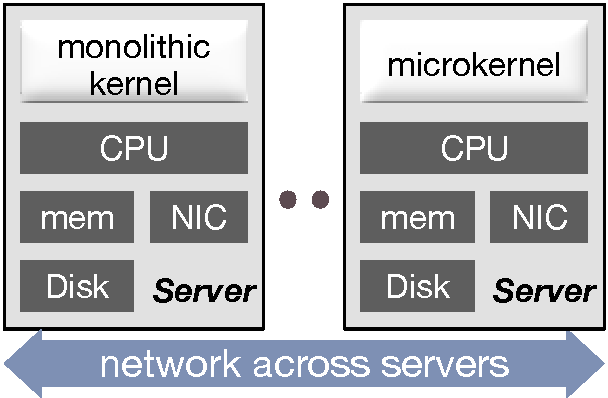
\includegraphics[width=1.7in]{lego/Figures/monolithic-arch.pdf}}
\caption[Monolithic OS.]{OSes Designed for Monolithic Servers.}
\label{fig-monolithic}
\end{center}
\end{subfigure}
\begin{minipage}{0.05in}
\hspace{0.05in}
\end{minipage}
\begin{subfigure}{1.8in}
\begin{center}
\centerline{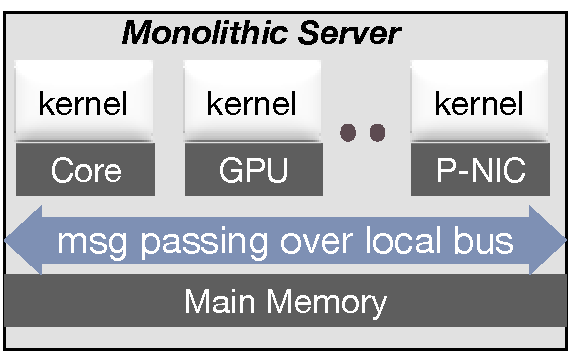
\includegraphics[width=1.8in]{lego/Figures/multikernel-arch.pdf}}
\caption[Multikernel Architecture.]{Multi-kernel Architecture. \small{P-NIC: programmable NIC.}}
\label{fig-multikernel}
\end{center}
\end{subfigure}
\begin{minipage}{0.05in}
\hspace{0.05in}
\end{minipage}
\begin{subfigure}{2.5in}
\begin{center}
\centerline{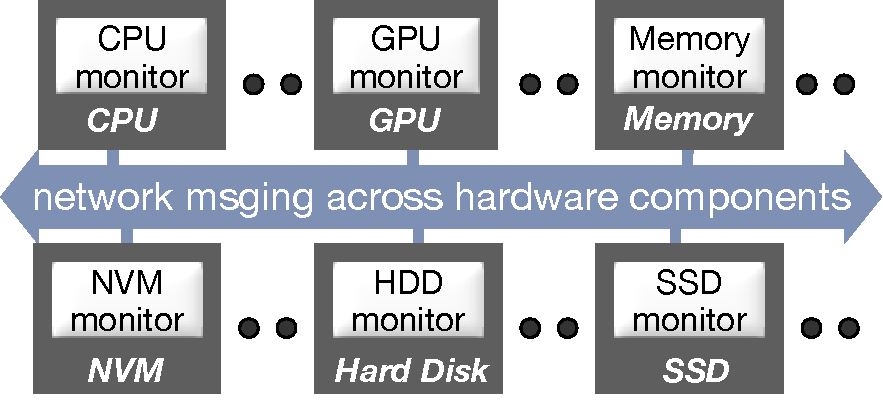
\includegraphics[width=2.6in]{lego/Figures/lego-arch.pdf}}
\caption[Splitkernel Architecture.]{Splitkernel Architecture.}
\label{fig-splitkernel}
\end{center}
\end{subfigure}
\caption[Operating System Architecture.]{Operating System Architecture.}
\end{figure*}
}

We propose {\em \splitkernel}, an OS architecture for hardware resource disaggregation (Figure~\ref{fig-architecture}).
The basic idea is simple: \textit{When hardware is disaggregated, the OS should be also}.  
A \splitkernel\ breaks traditional operating system functionalities into loosely-coupled {\em \microos{}s},
each running at and managing a hardware component
(\eg, a memory component's \microos\ runs at its hardware memory controller and allocates, protects, and virtualizes its hardware memory resources).
%and runs them on different hardware components. 
Monitors in a \splitkernel\ can be heterogeneous and can be added, removed, 
and restarted dynamically without affecting the rest of the system.
Each \splitkernel\ \microos\ can operate on its own for its own functionality and
only communicates with other \microos{}s when there is a need to access resources there.
There are only two global tasks a \splitkernel\ need to handle: 
orchestrating resource allocation across components 
and handling failure of components.


We choose not to support a general coherent view across different components in a \splitkernel.
Splitkernel does not assume or rely on a coherent network across hardware components.
All \microos{}s in a \splitkernel\ communicate with each other via {\em network messaging} only.
With our targeted scale, explicit message passing is much more efficient in network bandwidth consumption 
than the alternative of implicitly maintaining cross-component coherence.
%Building a \splitkernel\ is not as simple as just splitting an existing OS into separated pieces. 

Following the \splitkernel\ model, 
we built \lego, the {\em first} OS designed for hardware resource disaggregation.
%\lego\ is a distributed, loosely-coupled, failure-independent OS,
%designed and developed from scratch for disaggregated hardware architecture.
%\lego\ runs a {\em component manager} at each hardware component
\lego\ is a distributed OS that appears to applications as a set of virtual servers (called {\em \vnode{}s}).
A \vnode\ can run on multiple processor, memory, and storage components
and one component can host resources for multiple \vnode{}s.
%We use a two-level resource management mechanism for
\lego\ cleanly separates OS functionalities into %{\em micro OS services},
three types of {\em \microos{}s},
process \microos, memory \microos, and storage \microos. %to manage processes, memory, and storage data.
%Each \microos\ runs at the hardware component that it manages.
\lego\ \microos{}s share no or minimal states
and use a customized RDMA-based network stack to communicate with each other.
%\lego\ does not rely on or use any hardware-provided coherence across different hardware components.
%All \microos{}s in \lego\ communicate through explicit messaging over a customized RDMA-based network layer.
%manager, memory manager, and storage manager.
%\lego\ uses coarse-grained, global resource management to allocate, schedule, and coordinate across components. 
%Its design follows several principles.
%\lego\ currently consists of three types of \microos{}s to manage CPU, memory, and storage devices.

\if 0
\lego\ cleanly separates the functionalities of different component managers,
with zero or only minimal dependencies across them. 
This clean separation not only makes it easy to deploy, add, and remove components
but is also essential to ensuring failure independence. 
Our approach is to build each \lego\ manager as a {\em stateless}
service and managers communicate with requests that contain all the information needed to fulfill them.
For example, our storage manager is built in the NFS stateless server style~\cite{sun-nfs}.
\lego\ processor and memory managers are also cleanly separated 
in that memory managers manage all physical memory and virtual memory addresses, their allocation, deallocation, and mappings,
and processor only views virtual memory addresses assigned by memory managers. 
\fi

The biggest challenge and our focus in building \lego\ is the separation of processor and memory and their management.
Modern processors and OSes assume all hardware memory units including main memory, page tables, and TLB are local.
Simply moving all memory hardware and memory management software to behind network will not work.
%The simple separation of moving all memory function units behind network
%to manage disaggregated and distributed memory components
%and to provide good application performance when memory accesses are across the network. 

Based on application properties and hardware trends, 
we propose a hardware plus software solution that cleanly separates processor and memory functionalities,
while meeting application performance requirements.
\lego\ moves all memory hardware units to the disaggregated memory components
and organizes all levels of processor caches as virtual caches that are accessed using virtual memory addresses. 
To improve performance, \lego\ uses a small amount (\eg, 1\GB) of DRAM
organized as a virtual cache below current last-level cache.

\lego\ process \microos\ manages application processes and the extended DRAM-cache.
Memory \microos\ manages all virtual and physical memory space allocation and address mappings. 
\lego\ uses a novel two-level distributed virtual memory space management mechanism,
which ensures efficient foreground memory accesses and balances load and space utilization at allocation time.
Finally, \lego\ uses a space- and performance-efficient memory replication scheme to handle memory failure.
%with the observation that most applications already handle storage failure and our disaggregated architecture 
%mainly adds failure probabilities in memory.
%Replication in memory also has the benefits of sustain memory component failure in addition to processor failure. 
%We also port several drivers from Linux and implement both a customized, efficient network layer and the TCP/IP network stack.
%Overall, our goal is to run any binaries in \lego\ without any modifications. Hence we can
%port current distributed software ecosystem to \lego\ more smoothly.

We implemented \lego\ on the x86-64 architecture.
\lego\ is fully backward compatible with Linux ABIs
by supporting all common Linux system call APIs.
To evaluate \lego, we emulate disaggregated hardware components using commodity servers.
%For example, %to emulate a memory component, we only enable two cores of a server.
%to emulate a processor component, we limit the accessible physical memory of a server
%and use it as \lego's software-managed cache. 
%We are using InfiniBand as our high-speed network connection.
We evaluated \lego\ with microbenchmarks, the PARSEC benchmark~\cite{PARSEC}, %Filebench~\cite{Filebench},
and two unmodified datacenter applications, Phoenix~\cite{Ranger07-HPCA},
and TensorFlow~\cite{TensorFlow}.
%and an open-source MapReduce system called Phoenix~\cite{Ranger07-HPCA}.
Our evaluation results show that compared to monolithic Linux servers that can hold all the memory of these applications,
\lego\ is only 1.5\x\ to 1.7\x\ slower with around 25\% of application resident memory available as DRAM cache at processor components.
%running unmodified applications with \lego\ on a disaggregated cluster 
%is only 1.2\x to 2.1\x slower than running them on monolithic Linux servers that 
\lego\ outperforms monolithic Linux servers whose main memory size is 25\% of application resident memory 
and use local SSD/DRAM swapping (by 0.84\x\ to 3.0\x) or network swapping (by 0.97\x\ to 3.1\x). 
At the same time, \lego\ can improve resource packing %by up to XXX\x\
and reduce system mean time to failure. % by 18\% to 49\%.
%while potentially providing better support for hardware heterogeneity and elasticity.
%improves perf/\$ by 33\% to 66\% over monolithic Linux server, 
%with a typical disaggregated cluster ,
%while providing better support for heterogeneity, elasticity, resource utilization, and reliability.
% XXX \lego's performance is still worse than Linux and 
%we identified network delay being a major bottleneck.

Overall, this work makes the following contributions:

\begin{itemize}

\vspace{-0.05in}
\item We propose the concept of \splitkernel, an OS model that fits well with the hardware resource disaggregation architecture.

\vspace{-0.05in}
%\vspace{-0.1in}
\item We built \lego, the first OS that runs on and manages a disaggregated hardware cluster.
%designed for disaggregated systems.

\vspace{-0.05in}
%\vspace{-0.1in}
\item We propose a new hardware architecture to cleanly separate processor and memory hardware functionalities, 
while preserving most of the performance of monolithic server architecture.

\vspace{-0.05in}
%\vspace{-0.1in}
\item We presented a practical method to emulate disaggregated hardware and evaluate OS built for hardware resource disaggregation.
%and evaluated \lego\ with microbenchmarks and unmodified datacenter applications.
Our evaluation results of \lego\ shed light on future software and hardware directions in resource disaggregation.

\vspace{-0.05in}
%\vspace{-0.1in}

\end{itemize}

\lego\ is publicly available at {\small {\em {\url{http://LegoOS.io}}}}.\\

The rest of the paper is organized as follows.
\S{}2 motivates hardware resource disaggregation and a new OS for it.
\S{}3 presents the concept of \splitkernel.
We then discuss the detailed design and implementation of \lego\ in \S{}4 and \S{}5.
\S{}6 presents our evaluation results of \lego.
Finally, we cover related works in \S{}7 and conclude in \S{}8.

\section{Disaggregate Hardware Resource}
%\section{Disaggregate Hardware and OS}
\label{sec:motivation}

This section %discusses the limitations of monolithic servers
%in face of several datacenter trends and 
motivates the hardware resource disaggregation architecture
and discusses the challenges in managing disaggregated hardware.
%and shortages of existing OSes for that.
%We will present a full monetary cost model of our proposed resource disaggregation architecture 
%in \S~\ref{sec:cost}.

\subsection{Limitations of Monolithic Servers}
\label{sec:monolimit}
% why we must change and this is doomed for future!
A monolithic server has served as the unit of deployment and operation in datacenters
for decades. % (Figure~\ref{fig-monolithic}). 
%Several recent trends in datacenters are challenging 
However, this long-standing {\em server-centric} architecture has several key limitations.
%We believe that these trends will continue to exist in the future
%and we question {\em should datacenters continue to use monolithic servers?}

%\subsubsection{Inefficient Resource Utilization}
\noindent{\textit{\uline{Inefficient resource utilization.}}}
With a server being the physical boundary of resource allocation, 
it is difficult to fully utilize all resources in a datacenter~\cite{Barroso-COMPUTER,Quasar-ASPLOS,PowerNap}.
We analyzed two production cluster traces: a 29-day Google one~\cite{GoogleTrace}
and a 12-hour Alibaba one~\cite{AliTrace}.
Figure~\ref{fig-resource-anal} plots the aggregated CPU and memory utilization in the two clusters.
For both clusters, only around half of the CPU and memory are utilized.
Interestingly, %our analysis of the Google cluster (Figure~\ref{fig-google-evict}) shows that 
a significant amount of jobs are being evicted at the same time in these traces
(\eg, evicting low-priority jobs to make room for high-priority ones~\cite{Borg}). % (Figures~\ref{fig-googleevict} and \ref{fig-alievict}).
One of the main reasons for resource underutilization in these production clusters is 
the constraint that CPU and memory for a job have to be allocated from 
the same physical machine.
%The diversity and dynamism of today's datacenter workloads
%make resource allocation even more difficult.
%As a result, datacenters need to host more servers,
%costing more %(both CapEx and OpEx) 
%to meet application requirements.


\noindent{\textit{\uline{Poor hardware elasticity.}}}
%In a monolithic server architecture, %the processor-to-memory ratio is limited and 
It is difficult to add, move, remove, or reconfigure hardware components
after they have been installed in a monolithic server~\cite{FB-Wedge100}. %, and
Because of this rigidity, datacenters have to plan out server configurations in advance.
However, with today's speed of change in application requirements, such plans have to be adjusted frequently,
and when changes happen, it often comes with waste in existing server hardware.

{    
\begin{figure}[h]
\begin{subfigure}{2.5in}
    \begin{center}
    \centerline{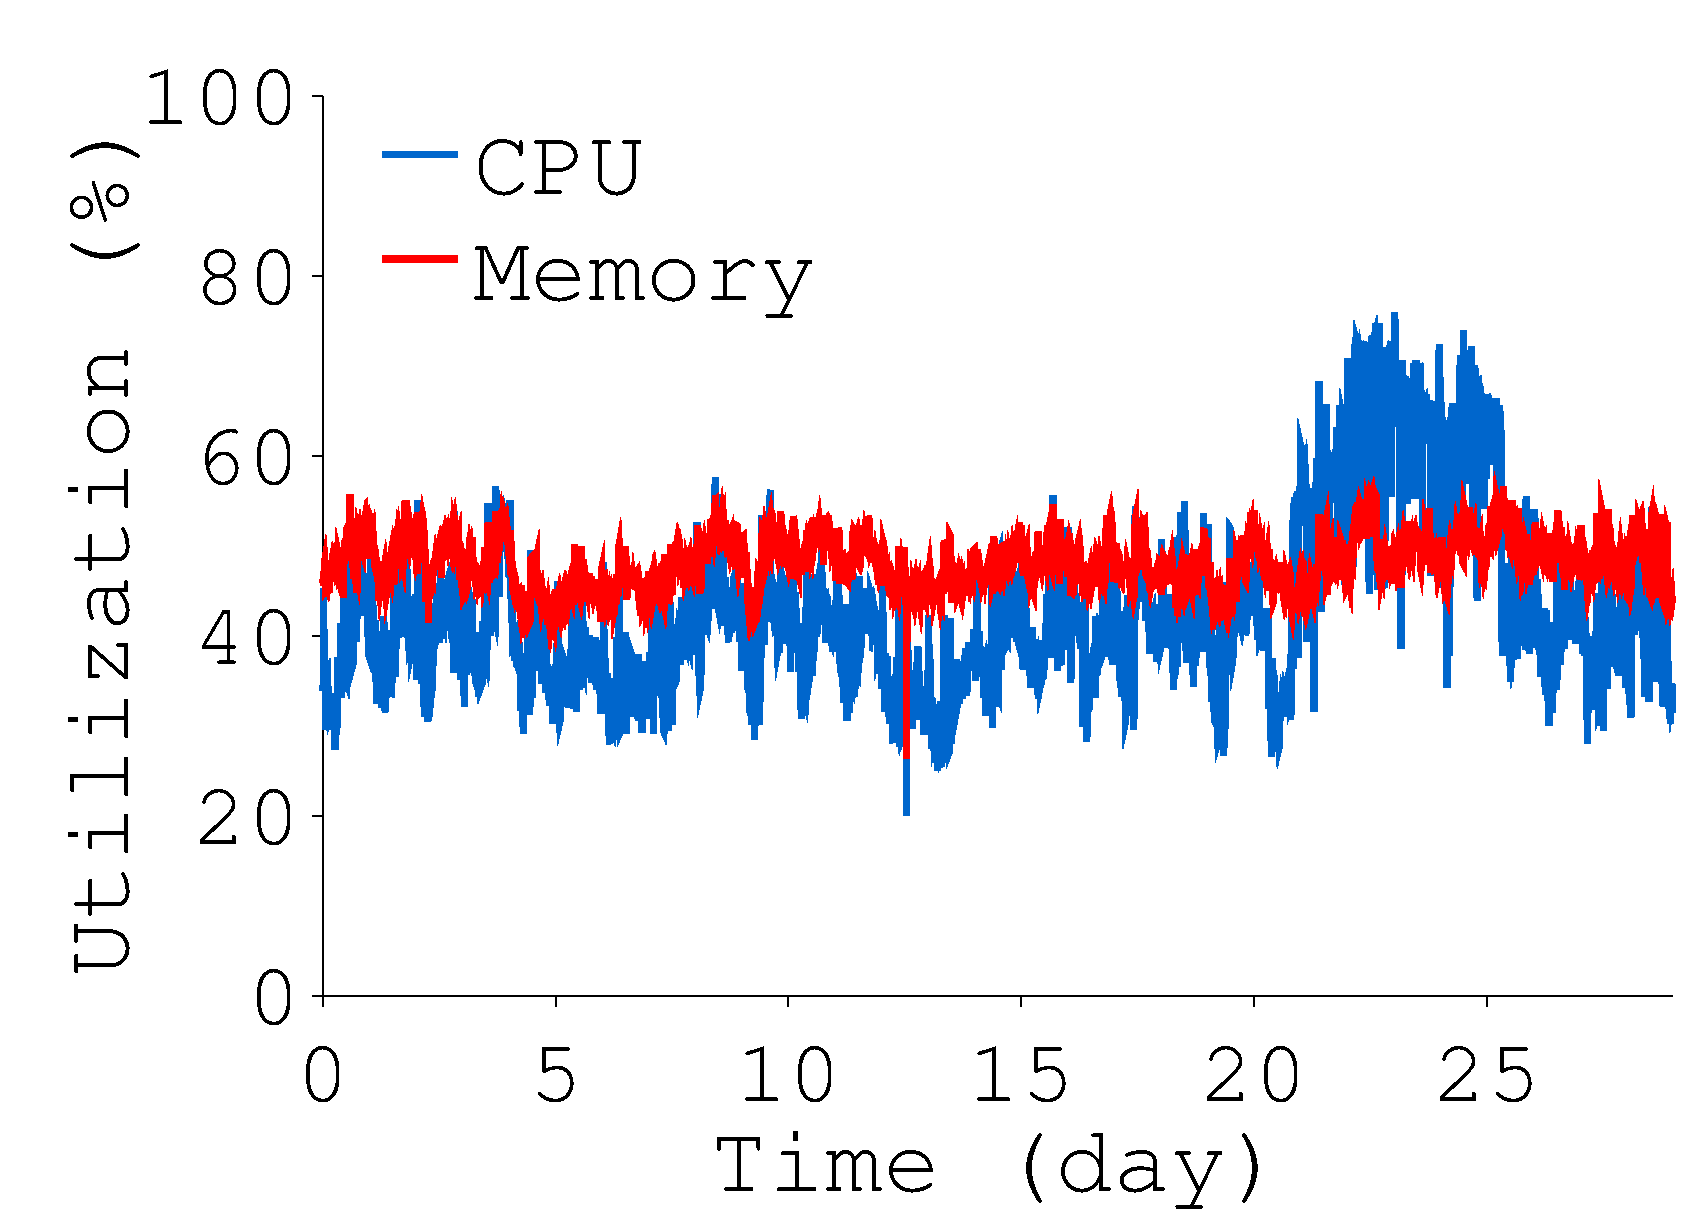
\includegraphics[width=2.5in]{lego/Figures/g_plot_google_util.pdf}}
    \caption[Google Cluster.]{Google Cluster.}
    \label{fig-googleutil}    
    \end{center}
\end{subfigure}
\begin{subfigure}{2.5in}
    \begin{center}    
    \centerline{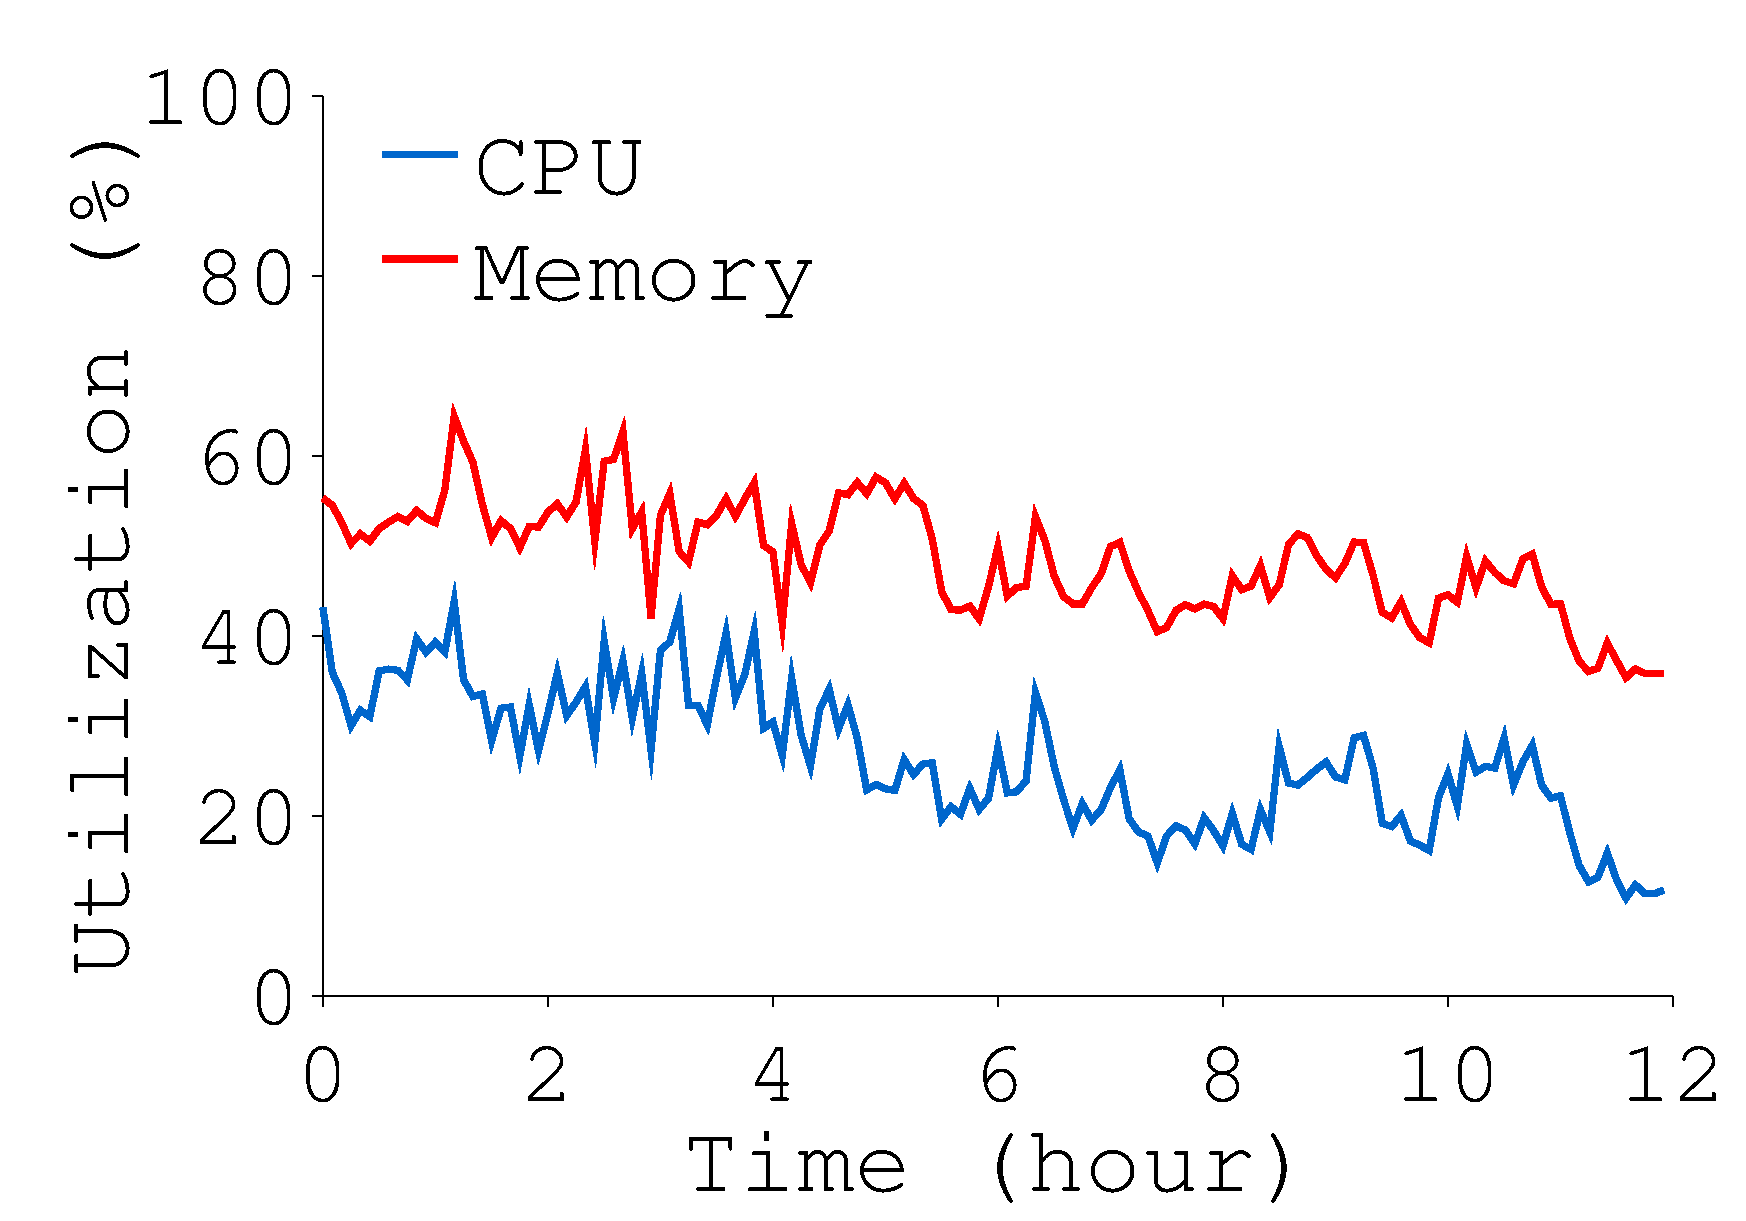
\includegraphics[width=2.5in]{lego/Figures/g_plot_ali_util.pdf}}    
    \caption[Alibaba Cluster.]{Alibaba Cluster.}
    \label{fig-aliutil}
    \end{center}    
\end{subfigure}
\caption[Data center resource utilization.]{Data center resource utilization.}
\label{fig-resource-anal}
\end{figure}
}
\noindent{\textit{\uline{Coarse failure domain.}}}
The failure unit of monolithic servers is coarse.
When a hardware component within a server fails, %(\eg, processor, memory chip, RAID controller), 
the whole server is often unusable and applications running on it can all crash.
Previous analysis~\cite{Failure-Disk-FAST07} found that motherboard, memory, CPU, power supply failures account for 
50\% to 82\% of hardware failures in a server.
Unfortunately, monolithic servers cannot continue to operate when any of these devices fail.

\if 0
\noindent{\textit{\uline{Hardware capacity wall.}}}
Pins, space, and power source in a monolithic server limit the capacity of hardware resource.
For example, the number of memory channels per socket~\cite{ITRS14} and DIMM density 
limit the memory capacity in a single server~\cite{HP-MemoryEvol,MemoryWall95,MemoryCube-ISCA17,Lim09-disaggregate}. 
As the number of cores per server increases, memory capacity is unable to keep pace.
Today's processor-to-memory ratio is already limiting the performance of datacenter applications~\cite{Ongaro11-RamCloud,page-graph}, 
forcing designers to resort to storage techniques~\cite{Zhang-FAST15-FlashGraph} 
or to scaling out~\cite{GU17-NSDI,Dragojevic14-FaRM,Dragojevic15-FaRM,Gonzalez12-OSDI}.
%Gonzalez-OSDI14-GraphX,Low-UAI10-GraphLab,Malewicz-SIGMOD10-Pregel,Kyrola-OSDI12-GraphChi}.
%Compounding the problem, data-intensive applications such as graph and deep learning~\cite{Gonzalez14-OSDI,Low12-VLDB,TensorFlow}
%require large amounts of memory.
\fi

\noindent{\textit{\uline{Bad support for heterogeneity.}}}
Driven by application needs, new hardware technologies are finding their ways into modern datacenters~\cite{sigarch-dc}.
Datacenters no longer host only commodity servers with CPU, DRAM, and hard disks. 
They include non-traditional and specialized hardware like GPGPU~\cite{GPU-google,GPU-aws}, 
%hardware technologies such as general-purpose GPU (GPGPU),
%specialized processors such as 
TPU~\cite{TPU}, 
%~\cite{DaDianNao,PuDianNao,PARD},
%and various FPGA and ASIC~\cite{Putnam14-FPGA},
DPU~\cite{DPU},
FPGA~\cite{Putnam14-FPGA,Amazon-F1}, %,SmartNIC-nsdi18},
%new and specialized memory components like Oracle 
non-volatile memory~\cite{Intel3DXpoint}, %,facebook-eurosys18},
%\yizhou{switch~\cite{FBOSS-SIGCOMM18,netcache-sosp17},}
%Program-In-Memory and Program-Near-Memory~\cite{Ahn15-PIM,Bojnordi12}.
%and new storage devices like 
and NVMe-based SSDs~\cite{everspin}.
%These hardware technologies have different performance, reliability, and energy-efficiency properties 
%that can benefit different applications.
%hardware and software heterogeneity
%
The monolithic server model tightly couples hardware devices with each other and with a motherboard.
As a result, making new hardware devices work with existing servers is a painful and lengthy process~\cite{Putnam14-FPGA}.
\if 0
System builders first need to design the interface for new devices to fit a specific bus or interconnect protocol.
They then have to find available slots in existing servers in a datacenter 
or purchase new servers to deploy the new devices.
Finally, system software like an OS may also need to change to utilize new hardware features.
With multiple new devices to be designed and deployed together, 
the problem becomes even worse, like {\em the matrix of hell}~\cite{Docker-PAAS}.
\fi
%
The current practice of making new hardware work is not only slow but also expensive.
%The common practice now is to build and deploy new servers for new hardware components. 
Datacenters often need to purchase new servers to host certain hardware.
Other parts of the new servers can go underutilized 
and old servers need to retire to make room for new ones.


\subsection{Hardware Resource Disaggregation}
The server-centric architecture is a bad fit for the fast changing datacenter hardware, software, and cost needs.
%Why virtual resource disaggregation is not enough?
There is an emerging interest in utilizing resources beyond a local machine~\cite{Gao16-OSDI},
such as distributed memory~\cite{Dragojevic14-FaRM,Nelson15-ATC,Aguilera17-SOCC,Novakovic16-SOCC} and network swapping~\cite{GU17-NSDI}. 
These solutions improve resource utilization over traditional systems.
However, they cannot solve all the issues of monolithic servers (\eg, the first three issues in \S\ref{sec:monolimit}), 
since their hardware model is still a monolithic one.
To fully support the growing heterogeneity in hardware and to provide elasticity and flexibility at the hardware level, 
we should {\em break the monolithic server model.}% into flexible resource components.

We envision a {\em hardware resource disaggregation} architecture 
where hardware resources in traditional servers are decomposed into disseminated, loosely-coupled, network-attached {\em components}.
Each component has its own controller and network interface
and is an {\em independent, failure-isolated} entity.

%benefits
The disaggregated approach largely increases the flexibility of a datacenter.
Applications can freely use resources from any hardware component,
which makes resource allocation easy and efficient.
Different types of hardware resources can {\em scale independently}.
It is easy to add, remove, or reconfigure components.
New types of hardware components can easily be deployed in a datacenter ---
by simply enabling the hardware to talk to the network and adding a new network link to connect it.
Finally, hardware resource disaggregation enables fine-grain failure isolation, % because of decomposed hardware resources.
since one component failure will not affect the rest of a cluster.

Three hardware trends are making resource disaggregation feasible in datacenters.
First, network speed has grown by more than an order of magnitude and has become more scalable in the past decade % faster both in bandwidth and latency
with new technologies like Remote Direct Memory Access ({\em \rdma})~\cite{ibverbs} 
and new topologies and switches~\cite{FireBox-FASTKeynote,costa15-r2c2,Costa-WRSC14},
enabling fast accesses of hardware components that are disaggregated behind network.
%Intel OmniPath~\cite{OmniPath}.
InfiniBand will soon reach 200Gbps and sub-500 nanosecond speed~\cite{Mellanox-ConnectX6,Mellanox-ConnectX6-IB,Mellanox-Switch},
being only 2\x\ to 3\x\ slower than main memory bus in bandwidth.
With main memory bus facing a bandwidth wall~\cite{BW-Wall-ISCA09},
future network bandwidth (at line rate) is even projected to exceed local DRAM bandwidth~\cite{CacheCloud-hotcloud18}.
%These network developments will enable fast accesses to disaggregated hardware. % even when crossing network.
%XXX check if 200Gbps is already available

Second, network interfaces are moving closer to hardware components,
with technologies like Intel OmniPath~\cite{OmniPath},
RDMA~\cite{ibverbs},
and NVMe over Fabrics~\cite{NVMe-fabrics-Inteltalk,NVMe-fabrics}.
As a result, hardware devices will be able to access network directly 
without the need to attach any processors. 

Finally, hardware devices are incorporating more processing power~\cite{Ahn15-PIM,Bojnordi12,Mellanox-SmartNIC,Mellanox-SmartNIC2,Agilio-SmartNIC,Junwhan-ISCA17},
allowing application and OS logics to be offloaded to hardware~\cite{Willow,Kaufmann16-ASPLOS}.
On-device processing power will enable system software to manage disaggregated hardware components locally.

With these hardware trends and the limitations of monolithic servers,
we believe that datacenters should start to seek options in hardware resource disaggregation.
In fact, there have already been several initial hardware proposals in resource disaggregation~\cite{OCP},
including disaggregated memory~\cite{Lim09-disaggregate,Scaleout-numa}, 
disaggregated flash~\cite{FlashDisaggregation,ReFlex},
new power state for disaggregated memory~\cite{Nitu18-EUROSYS},
Intel Rack-Scale System~\cite{IntelRackScale}, 
HP ``The Machine''~\cite{HP-TheMachine,HP-MemoryOS}, 
IBM Composable System~\cite{IBM-Composable},
and Firebox~\cite{FireBox-FASTKeynote}.


\subsection{OS for Resource Disaggregation}
Despite various benefits hardware resource disaggregation promises, 
it is still unclear how to manage or utilize disaggregated hardware in a datacenter.
Unfortunately, existing OSes and distributed systems cannot work well with this new architecture.
Single-node OSes like Linux view a server as the unit of management and assume all hardware components are local (Figure~\ref{fig-monolithic}).
A potential way to use them with hardware resource disaggregation is to run them on processors
and access memory, storage, and other hardware resources remotely.
Recent disaggregated systems like soNUMA~\cite{Scaleout-numa} take this approach.
However, this approach incurs higher network latency and bandwidth consumption with remote device management,
misses the opportunity of exploiting device controller computation power,
and makes processors the point of failure.
%They cannot handle hardware components that are separated by the network.

Multi-kernel solutions~\cite{Baumann-SOSP09,Barrelfish-DC,Helios-SOSP,fos-SOCC,Hive-SOSP} (Figure~\ref{fig-multikernel}) 
view different cores, processors, or programmable devices within a server separately 
by running a kernel on each core/device and using message passing to communicate across kernels.
%Multi-kernel OSes fit better to hardware resource disaggregation than monolithic kernels.
These kernels still run in a single server and all access some common hardware resources in the server like memory and network interface to outside.
Moreover, they do not manage distributed resources or handle failures in a disaggregated cluster. 
%The multi-kernel architecture fits better with hardware resource disaggregation
%However, multi-kernels still manage memory and storage as a whole in a monolithic server.
%Other single-node OS proposals focus on improving flexibility~\cite{Exokernel,Drawbridge}, scalability~\cite{Corey-OSDI,Disco,K42-EUROSYS}, security~\cite{SealingOS}.
%None of these existing OSes handle the distributed nature of hardware resource disaggregation.

There have been various distributed OS proposals,
most of which date decades back~\cite{Amoeba-Experience,Sprite,MOSIX}. %,V-System,Accent-SOSP,DEMOS-SOSP,Charlotte}.
%The idea of building distributed operating systems is not new and has been explored decades ago.
%Sprite~\cite{}, Amoeba~\cite{Amoeba-Status,Amoeba-Experience}, V~\cite{}, MOSIX~\cite{}, Accent~\cite{}, Charlotte~\cite{}, DEMOS are
Most of these distributed OSes manage a set of monolithic servers
instead of hardware components.

Hardware resource disaggregation is fundamentally different from the traditional monolithic server model.
A complete disaggregation of processor, memory, and storage 
means that when managing one of them, there will be no local accesses to the other two.
For example, processors will have no local memory or storage to store user or kernel data.
Memory and storage components will only have limited processing power. %not have no local memory to serve as cache.
%If we run an OS only at processors, it will need to remotely manage all other components, causing high network overhead.
OS also needs to manage a distributed set of resources and handle their failure.
%Clearly, hardware resource disaggregation calls for a redesign of OS.
%What makes today's disaggregated os different is advances in network and hardware heterogeneity?
%on the other hand, there are new constraints and challenges
%We believe that now is the time to reconsider how OS.. build a new OS
%\subsection{Challenges in Managing Disaggregated Resources}
%Hardware resource disaggregation completely shifts the paradigm of computer hardware and software systems
We identified the following key challenges in building an OS to manage a disaggregated cluster,
%and presents many new challenges,
some of which have previous been identified~\cite{HP-MemoryOS}.

\begin{itemize}
\vspace{-0.05in}
\item How to deliver good performance when application execution involves the access of network-partitioned disaggregated hardware
and currently network is still slower than local buses?

\vspace{-0.05in}
\item How to locally manage individual hardware components with limited hardware resources?

%\item How to communicate across components?

\vspace{-0.05in}
\item How to manage distributed hardware resources efficiently?

\vspace{-0.05in}
\item How to handle the failure of a component without affecting other components and running applications?

\vspace{-0.05in}
\item What abstraction should be exposed to users and how to support existing datacenter applications?

\vspace{-0.05in}
\end{itemize}

Instead of retrofitting existing OSes to confront these challenges,
we took the approach of designing a new OS architecture from the ground up for hardware resource disaggregation.

\if 0
\noindent{\textit{\uline{Latency performance.}}} %of accessing components over network.}}}
Although network bandwidth is now approaching and could exceed PCIe and memory bus bandwidth in the
future, network latency is still XXX slower.
How can a disaggregated cluster deliver good performance
%When hardware is disaggregated across network,
%it is inevitable to involve network communication during application execution.
%The biggest challenge in building a \splitkernel\ is the separation of processors and memory.
%With current network still being ~5\x\ slower in bandwidth and ~50\x\ slower in latency than memory bus, 
%if all memory accesses are cross the network, 
%application performance will be significantly impacted.

\noindent{\textit{\uline{How to manage distributed hardware resources.}}}
We envision the scale of a disaggregated cluster to be at least one rack, 
hosting hundreds of hardware components.
Managing them are different from traditional....
%To be fully flexible and elastic, applications should be able to utilize resources
%from any components.
%A \splitkernel\ thus needs an efficient mechanism to allocate and manage 
%hardware resources in a disaggregated cluster for different applications.

\noindent{\textit{\uline{Failure handling.}}} %How to handle hardware failures?}}}
Hardware resource disaggregation has both positive and negative implications in reliability.
The failure of disaggregated hardware will not affect other hardware.
But the total number of network-attached components can increase after disaggregation (\S\ref{sec:cost})
and each hardware component can host resources for multiple applications.
%The reliability of a disaggregated cluster largely depends on how
%software manages it and such failure handling should not come with a high 
%space or performance overhead.

\noindent{\textit{\uline{How to support existing datacenter applications?}}}
%Being able to easily port existing datacenter applications is crucial to the adoption of a \splitkernel.
%However, all current datacenter applications are designed to run on monolithic servers.
%To provide complete transparency and backward compatibility, 
%\splitkernel\ should hide the resource disaggregation nature. % in a disaggregated OS.

\noindent{\textit{\uline{Managing individual hardware component.}}} %How to manage individual hardware components with hardware constraints?}}}
%To support heterogeneity and failure independence, 
Each component in a disaggregated cluster should operate on its own as much as possible.
Thus, each \microos\ should manage its own hardware component
without involving other \microos{}s or network communication to them.
A major challenge in achieving this goal is that no component is a full-fledged server. 
They lack hardware resources that OSes and applications traditionally assume to be local.

\fi
\section{The Splitkernel OS Architecture}
\label{sec:design}

We propose {\em \splitkernel}, a new OS architecture for resource disaggregation. 
Figure~\ref{fig-architecture} illustrates \splitkernel's overall architecture.
As suggested by its name, the main idea of \splitkernel\ is to disseminate an OS 
into pieces of different functionalities.
Apart from this main idea, we propose three concepts in \splitkernel:
each disseminated piece of \splitkernel\ runs at the hardware component it manages;
all components communicate by message passing over a common network;
and \splitkernel\ globally manages resources and component failures.
%and push each of them to run on a hardware component.
%\textit{{when hardware is disaggregated, the OS should be also}}.
%This section defines the \splitkernel\ architecture and its abstraction to users.
%All hardware components in a \splitkernel\ are connected to a general network and 
Splitkernel is a general OS architecture we propose for hardware resource disaggregation.
There can be many types of implementation of \splitkernel.
Further, we make no assumption on the specific hardware or network type in a disaggregated cluster \splitkernel\ runs on.
Below, we describe the four key concepts of \splitkernel\ in details.
%hardware model

%\subsection{Architecture and Abstraction Overview}
\noindent{\textit{\uline{Split OS functionalities.}}}
Splitkernel breaks traditional OS functionalities into {\em \microos{}s}.
Each \microos\ manages a hardware component, virtualizes and protects its physical resources.
\microos{}s in a \splitkernel\ are loosely-coupled and 
they communicates with other \microos{}s to access their resources. 
%deploys them at individual hardware components.
%\noindent{\textit{\uline{Use hints to improve performance.}}
%\noindent{\textit{\uline{Cleanly separate OS functionalities with no or minimal state sharing.}}}
%Resource disaggregation makes it possible to flexibly deploy heterogeneous hardware devices. 
%Hardware resource disaggregation enables different hardware components to run and fail on their own.
%To retain the benefits of disaggregated hardware, 
For each \microos\ to operate on its own with minimal dependency on other \microos{}s,
we use a stateless design by sharing no or minimal {\em states}, or metadata,
across \microos{}s.
%However, a clean separation is hard, especially when every hardware component has limited amount of resources.
%Sometimes, it even requires hardware changes (\S\ref{sec:hardware}).
%However, we can only obtain the benefits 
%if the software managing these hardware devices also provides good support for flexibility, elasticity, and heterogeneity.
%To achieve the same level of hardware disaggregation in software, 


\noindent{\textit{\uline{Run \microos{}s at hardware components.}}}
We expect each non-processor hardware component in a disaggregated cluster to have a controller that 
can run a \microos.
A hardware controller can be a low-power general-purpose core, an ASIC, or an FPGA.
Each \microos\ in a \splitkernel\ can use its own implementation to manage the hardware component it runs on.
This design makes it easy to integrate heterogeneous hardware in datacenters ---
to deploy a new hardware device, its developers only need to build the device,
implement a \microos\ to manage it, % and communicate with the rest of \splitkernel,
and attach the device to the network. 
Similarly, it is easy to reconfigure, restart, and remove hardware components with \splitkernel.
%A \microos\ can be added, restarted, or stopped dynamically without affecting the rest of the OS.

\noindent{\textit{\uline{Message passing across non-cache-coherent components.}}}
Unlike other proposals of disaggregated systems~\cite{HP-TheMachine} that rely on coherent interconnect~\cite{GenZ,ccix,OpenCAPI},
a \splitkernel\ runs on general-purpose network layer like Ethernet and 
neither underlying hardware or the \splitkernel\ provides cache coherence across components.
We made this design choice mainly because maintaining coherence for our targeted cluster scale 
would cause network bandwidth consumption.
% significant network bandwidth for coherence traffic.
Instead, all communication across components in a \splitkernel\ is through {\em network messaging}.
A \splitkernel\ still retains the coherence guarantee that hardware already provides within a component (\eg, cache coherence across cores in a CPU),
and applications running on top of a \splitkernel\ can use message passing to implement their desired level of coherence for their data across components.

\noindent{\textit{\uline{Global resource management and failure handling.}}}
One hardware component can host resources for multiple applications and its failure can affect all these applications.
In addition to managing individual components, \splitkernel\ also needs to 
globally manage resources and failure.
To minimize performance and scalability bottleneck,
\splitkernel\ only involves global resource management occasionally for coarse-grained decisions, 
%\splitkernel\ uses a two-level resource management mechanism, 
%where a global manager performs coarse-grained decisions 
while individual \microos{}s make their own fine-grained decisions.
\splitkernel\ handles component failure by adding redundancy for recovery.
%\noindent{\textit{\uline{Handle failure with minimal space and performance overhead.}}}
%Isolating and recovering from failure is important
%but should not come at the cost of high performance or memory space overhead during failure-free periods. 
%For example, a full replication on every memory access would be costly both in space and in performance.
%Our idea is to reduce full replication costs by performing partial, best-effort replication
%and re-use the already existing application-provided failure handling mechanisms.



%include abstraction??? XXX
\if 0
\splitkernel appears to users as a distributed set of 
%\noindent{\textit{\uline{Appear as a cluster of nodes.}}}
A disaggregated cluster can appear as one giant machine by hiding all its distributed components from users~\cite{Amoeba-Experience};
it can also expose all the disaggregated hardware components to users.
We choose an abstraction in between: users view a distributed set of nodes that \splitkernel\ exposes,
and \splitkernel\ hides the hardware disaggregation nature from users.
Most existing datacenter applications are built with the knowledge of distributed servers.
Maintaining the distributed view can seamlessly support all these existing distributed datacenter applications.
Moreover, it lets us reuse application-provided failure handling and message passing (\S\ref{sec:failure}).

\splitkernel\ not only manages individual hardware components but also orchestrates the communication
among components, manages their failure, and globally allocates resources across hardware components.
Combining all \microos{}s, \splitkernel\ is a distributed OS that manages all hardware components in a disaggregated cluster.
%in a disaggregated datacenter.
\fi

% XXX benefits
%Unlike many tightly-coupled existing OSes, \splitkernel's design of disaggregating OS functionalities
%not only makes it easy to deploy, add, and remove components
%but is also essential to achieving heterogeneity and ensuring failure independence. 
%No additional distributed system layer or hardware controllers are needed.
%, nor is any hardware controller.
%Figure~\ref{fig-architecture} illustrates the overall architecture of \splitkernel. 

%can have different types of memory, e.g., some use 4K page, some use huge page, some use segmentation
%different TLB impl
%applications can choose different memory device for their own needs
%can fail independently


%Internally, \splitkernel\ consists of a distributed set of disaggregated hardware components
%and can map different amount of hardware resources as one ``node'' to the application dynamically.

%However, as we will show in Section~\ref{sec:design}, 
%a clean separation of OS functionalities is hard and can sometimes come with tradeoffs in performance.


\if 0
\splitkernel\ is far from just decomposing an OS. 
A main challenge it needs to solve is to handle failure 
With the scale of \dcrack, failures are inevitable
Our goal is to 

contrary to current practice of not replicating memory, we believe that memory can and should be replicated. 
more memory space with disaggregated memory, no memory wall
has to handle memory failure
memory access already cross network, replication will not add too much cost
can also be used to improve parallelism
Given our planned scale of hardware components, failures are inevitable.
%a hardware component may fail, the software running on it may crash, or the network to it may fail or be too slow. 
When monolithic computers experience a hardware or OS crash, they typically terminate entire applications~\cite{Depoutovitch10-otherworld}.
However, many datacenter applications require high availability~\cite{MongoDB} or are long running~\cite{TensorFlow},
and it would be unacceptable to terminate a whole application when one part of the disaggregated system fails.
Since an application running on disaggregated architecture
can be using a set of hardware components and one component can host multiple applications, 
a component failure should not affect application execution or make the whole system unavailable.
\splitkernel\ needs to isolate failures and quickly recover from them. %offer even under failure scenarios.
Moreover, such approach should not come at a high cost of space overhead.
In particular, a memory space overhead of 2\x\ (\eg, the result of a full two-way memory content replication) 
can be prohibitive to datacenters that desire low monetary costs.
\fi

%We will seek various ways to reduce this overhead while still delivering our failure guarantees.

%We envision the scale of disaggregated architecture to have at least thousands of components.
%With this scale, failure is inevitable. 

%It will first need an efficient mechanism to collect resource utilization information,
%to execute resource management tasks, and to communicate across hardware components.
%Such mechanism should be low latency, consume minimal network bandwidth, and use small amount of space to store metadata.
%\lego\ then needs to deploy a set of good policies of global resource allocation and scheduling.



\if 0
\noindent{\textit{\uline{Minimize network communication}}
delay allocation
prefetching
piggy-back

\noindent{\textit{\uline{Layered Abstraction}}
our design only specifies the abstraction of each layer and interface between components
how each service is implemented is flexible and can be heterogeneous.

\noindent{\textit{\uline{Separate Policy from Mechanism}
Global Resource Management
different types of resources can register with the global resource manager
\fi


\if 0
For example, memory protection should be enforced at the memory side for a clean separation of functionality.
However, performing an early protection check at the processor side can avoid sending
unnecessary traffic (protection violations) to memory.
As another example, 
To cleanly separate components, we will build each manager 
as a {\em stateless} service and different managers communicate
with requests that contain all the information needed to fulfill them.
For example, a memory access request or a storage I/O request sent from a processor will 
include all the information the memory component or the storage component will need to fulfill the requests,
without the need to store any historical states at these components.
This stateless design will also make failure handling easier, 
since during recovery components do not need to restore states. 

The first decision we made to build \lego\ is to cleanly separate 
pluggable, heterogeneous implementation

clean separation from hardware to system software
%\noindent{\textit{\uline{Stateless Control}
long-running, non-user-interactive applications

processor only sees virtual memory addresses

user space code only running on processors, 
all other components run only one mode that is privileged, equivalent to kernel mode.

the decision of using only virtual memory address at processors has its own tradeoffs.

\noindent{\textit{\uline{Run OS services at hardware}}
Our next idea of \splitkernel\ is to run micro-OS services at individual hardware.
%why

challenge: limited hardware resources
%\noindent{\textit{\uline{How to meet hardware constraints?}}
%The \dcrack\ architecture 
Running \splitkernel\ services on hardware components raise new design and implementation challenges,
because each type of these components have their new constraints.
Processors will only have limited memory, 
while other types of resource components like memory and storage devices will only have limited processing power.
There will also be no local persistent storage for processors or memory to use.

%\noindent{\textit{\uline{How to cleanly separate OS services?}}
Different hardware components have different constraints.
For example, memory components will have plenty of memory but has limited processing power,
usually just a memory controller,
while processors will have limited amount of memory.
The disaggregated OS component manager should be designed with these constraints in mind.
Different managers should also be cleanly separated in their functionalities
and should have zero or minimal dependencies.
\fi

\if 0
\subsection{Challenges}
There are three main challenges in building a disaggregated OS:

\noindent{\textit{\uline{How to provide good application performance when hardware accesses are across the network?}}
Current datacenters and future racks will be able to host thousands of hardware components~\cite{HP-Moonshot,HP-m800},
the scale that we target to support.
This scale offers applications great parallelism.
However, the disaggregated approach inevitably adds a performance cost in network communication.
Managing thousands of distributed components may also create performance overhead. %could also introduce performance overhead. %There is also 
How to minimize or hide these costs is crucial to the success of \lego.


\noindent{\textit{\uline{How to support existing datacenter applications?}}
%All current datacenter applications are designed to run on monolithic servers.
%To provide complete transparency and backward compatibility, 
%we need to hide the resource disaggregation nature in a disaggregated OS.
%However, doing so can lead to reduced flexibility in resource management. 
%Applications need a transparent and user-familiar abstraction.
There is a host of popular datacenter applications~\cite{TensorFlow,Gonzalez14-OSDI,Malewicz10-SIGMOD,Kyrola12-OSDI,Low10-UAI,Low12-VLDB,Gonzalez12-OSDI,MongoDB}.
Being able to easily port these existing applications and efficiently run them will assist in the adoption of \lego.
%\myitemit{Q5: How to support existing datacenter applications?}
%Applications need a transparent and user-familiar abstraction.
However, all current datacenter applications are designed to run on monolithic servers.
To provide complete transparency and backward compatibility, 
we need to hide the resource disaggregation nature in a disaggregated OS.
%However, doing so can lead to reduced flexibility in resource management. 
%Workload or jobs will be distributed across different running instances in different
%computers. With a new unified-interface exposed by disaggregated operating system to represent
%all available hardware components, the model to run distributed systems is changed.

\fi
\section{\lego\ Design}
\label{sec:design}

Based on the \splitkernel\ architecture,
we built {\em \lego}, the first OS designed for hardware resource disaggregation.
\lego\ is a research prototype that demonstrates the feasibility of \splitkernel,
but it is not the only way to build a \splitkernel\ OS.
\lego's design targets three types of hardware components:
processor, memory, and storage,
and we call them {\em \pcomponent, \mcomponent}, and {\em \scomponent}.

This section first introduces the abstraction \lego\ exposes to users
and then describes the hardware architecture of components \lego\ runs on.
Next, we explain the design of \lego' process, memory, and storage \microos{}s.
We end this section with the discussion of \lego' global resource management and failure handling mechanisms.

Overall, \lego\ achieves the following design goals:

\begin{itemize}

%\vspace{-0.1in}
%\item Great support for hardware disaggregation which in turn offers heterogeneity, elasticity, and flexibility.
\vspace{-0.1in}

\item Clean separation of process, memory, and storage functionalities.
\vspace{-0.1in}

\item Runs at hardware components and fits well to device constraints.
%requires small hardware resources and can be easily deployed on hardware. 
\vspace{-0.1in}

\item Comparable performance as monolithic Linux servers.
\vspace{-0.1in}

\item Efficient resource management and memory failure handling, both in space and in performance. % and performance-efficient memory replication scheme.
\vspace{-0.1in}

\item Easy-to-use, backward compatible user interface.
\vspace{-0.1in}

\item Supports common Linux system call interfaces.
\vspace{-0.1in}

\end{itemize}

\subsection{Abstraction and Usage Model}
\lego\ exposes a distributed set of {\em virtual nodes}, or {\em \vnode}, to users.
From users' point of view, a \vnode\ is like a virtual machine. 
Multiple users can run in a \vnode\ and each user can run multiple processes.
Each \vnode\ has a unique ID, a unique virtual IP address, %({\em \vip}),
and its own storage mount point. % ({\em \vmount}).
\lego\ protects and isolates the resources given to each \vnode\ from others.
Internally, one \vnode\ can run on multiple \pcomponent{}s, multiple \mcomponent{}s,
and multiple \scomponent{}s.
At the same time, each hardware component can host resources for more than one \vnode.
The internal execution status is transparent to \lego\ users;
they do not know which physical components their applications run on.
%why

With \splitkernel's design principle of components not being coherent,
\lego\ cannot execute application threads that need to have shared write access to common memory.
\lego\ assumes threads within the same process to need shared write access
and threads belonging to different processes to not use shared writable memory,
and \lego\ makes scheduling decision based on this assumption (\S\ref{sec:proc-scheduling}).
Applications that use shared writable memory across processes (\eg, with MAP\_SHARED)
will need to change to use message passing across processes instead.
We made this decision because writable shared memory across processes is rare 
(we have not seen a single instance in the applications we studied),
and supporting it makes both hardware and software more complex 
(in fact, we have implemented this support but later decided to not include it because of its complexity).
%it needs to use a special flag to inform \lego\ at process creation time,
%so that \lego\ will schedule these processes at the same \pcomponent.

\if 0
%As discussed in Section~\ref{sec:principles}, we will 
\lego\ provides a non-cache-coherent interface across \pcomponent{}s.
Thus, we do not support writable memory sharing across \pcomponent{}s
and do not split a process across multiple \pcomponent{}s
(\lego\ allows read-only sharing, since it will not cause coherence issues).
Using process as the unit of deployment across \pcomponent{}s is sufficient. % and desired for existing datacenter applications,
Among the applications we studied, none use any inter-process {\em writable} memory sharing
Other studies~\cite{OVC} also show that inter-process sharing of writable in-memory data is rare.
Although \lego\ does not share (writable) memory across \pcomponent{}s, 
different \pcomponent{}s can use separate physical memory spaces on the same \mcomponent.
\fi

One of the initial decisions we made when building \lego\ is to support Linux system call interface 
and unmodified Linux ABI,
because doing so can greatly ease the adoption of \lego.
Distributed applications that run on Linux can seamlessly run on a \lego\ cluster
by requesting a set of \vnode{}s from \lego\ and use their virtual IP addresses to communicate.
%Applications that fit well to \lego\ are computation intensive 
%or exhibit fairly good memory locality;
%many datacenter applications fall into this category~\cite{TensorFlow,Gonzalez12-OSDI,XXX}.
%We do not target storage-intensive applications currently and leave the 
%optimization of disaggregated storage for future work.

{
\begin{figure*}[th]
\begin{minipage}{\figWidth}
\begin{center}
\centerline{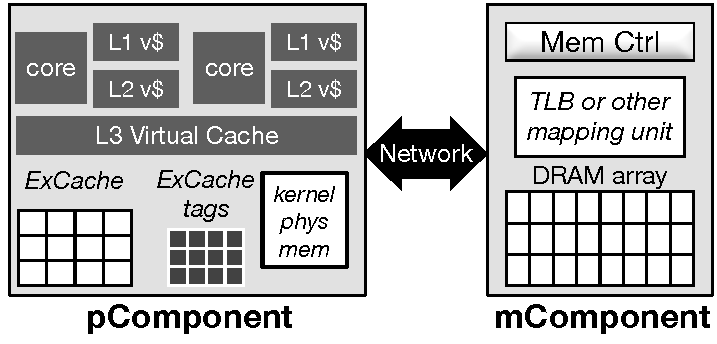
\includegraphics[width=2.8in]{Figures/hwarch.pdf}}
\vspace{-0.1in}
\mycaption{fig-hw-arch}{\lego\ \pcomponent\ and \mcomponent\ Architecture.}
{
}
\end{center}
\end{minipage}
\begin{minipage}{0.05in}
\hspace{0.05in}
\end{minipage}
\begin{minipage}{\figWidth}
\begin{center}
\centerline{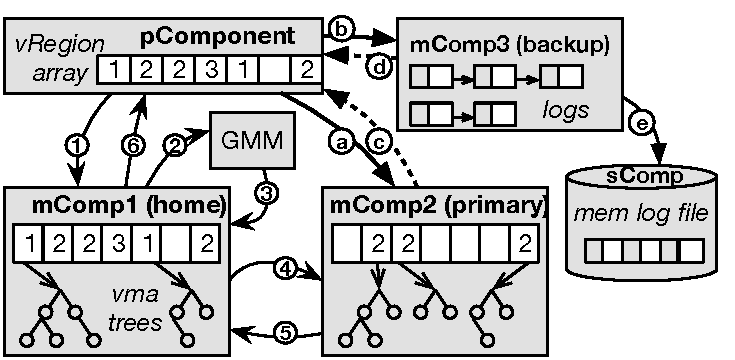
\includegraphics[width=2.8in]{Figures/dist-vma.pdf}}
\vspace{-0.1in}
\mycaption{fig-dist-vma}{Distributed Memory Management.}
{
}
\end{center}
\end{minipage}
\vspace{-0.15in}
\end{figure*}
}

\subsection{Hardware Architecture}
\label{sec:hardware}
\lego\ \pcomponent, \mcomponent, and \scomponent\ are independent devices,
each having its own hardware controller and network interface (for \pcomponent, the hardware controller is the processor itself).
Our current hardware model uses CPU as the processor in \pcomponent, 
DRAM in \mcomponent, and SSD or HDD in \scomponent.
We leave the exploration of other hardware devices for future work.

%\splitkernel\ views each hardware component as an independent unit connected to a global network
%and it is not specific to any hardware device architecture.
%Splitkernel supports hardware heterogeneity and allows different hardware architectures to work in a disaggregated cluster.
To demonstrate the feasibility of hardware resource disaggregation,
we propose a \pcomponent{} and a \mcomponent\ architecture designed 
within today's network, processor, and memory performance and hardware constraints
(Figure~\ref{fig-hw-arch}).

\noindent{\textit{\uline{Separating process and memory functionalities.}}}
\lego\ moves all hardware memory functionalities to \mcomponent{}s 
(e.g., page tables, TLBs) and leaves {\em only} caches at \pcomponent{} side. 
With a clean separation of process and memory hardware units, 
the allocation and management of memory can be completely transparent to \pcomponent{}s.
Each \mcomponent{} can choose their own memory allocation technique
and virtual to physical memory address mappings (\eg, segmentation). 
A side benefit of moving TLB to \mcomponent{} is that \pcomponent{} cache accesses would not 
need to wait for TLB results~\cite{Kaxiras-ISCA13}, potentially making \pcomponent{}s run faster.
%reason for moving TLB: TLB miss cost would be high and cite ASPLOS'18 paper on why TLB miss can be frequent

\noindent{\textit{\uline{Processor virtual caches.}}}
After moving all memory functionalities to \mcomponent, %including memory address mapping to memory, 
\pcomponent{}s will only see virtual addresses and have to use virtual memory addresses to access its caches. 
Because of this, \lego\ organizes all levels of \pcomponent{} caches as {\em virtual caches}~\cite{Goodman-ASPLOS87,Wang-ISCA89},
\ie, virtually-indexed and virtually-tagged caches.

A virtual cache has two potential problems, commonly known as synonyms and homonyms~\cite{CacheMemory82}.
Synonyms happens when a physical address maps to multiple virtual addresses (and thus multiple virtual cache lines) 
as a result of memory sharing across processes,
and the update of one virtual cache line will not reflect to other lines that share the data.
Since \lego\ does not allow writable inter-process memory sharing,
it will not have the synonyms problem.
The homonyms problem happens when two address spaces use the same virtual address for their own different data.
Similar to previous solutions~\cite{OVC}, we solve homonyms by storing an address space ID (ASID) with each cache line,
and differentiate a virtual address in different address spaces using ASID.

\noindent{\textit{\uline{Separating memory for performance and for capacity.}}}
Previous studies~\cite{Gao16-OSDI,GU17-NSDI} and our own show that today's network speed 
cannot meet application performance requirements if all memory accesses are behind the network. 
Fortunately, many modern datacenter applications exhibit strong memory access temporal locality.
For example, we found 90\% of memory accesses in PowerGraph~\cite{Gonzalez12-OSDI} go to just 0.06\% of total memory
and 95\% go to 3.1\% of memory
(22\% and 36\% for TensorFlow~\cite{TensorFlow} respectively
and 5.1\% and 6.6\% for Phoenix~\cite{Ranger07-HPCA}).
%PG 90% 0.0063G 95% 0.301G 100% 9.68G
%TF 90% 0.608G 95% 0.968G 100% 2.7G
%There is a clear separation of applications' working sets that are frequently accessed 
%and the rest of their memory footprints that are large but rarely accessed.
% XXXgive TF mem access pattern
%batch size

With good memory-access locality, we propose to %separate hardware memory into two categories and organize them differently:
leave a small amount of fast memory (\eg, 1\GB) at each \pcomponent{}
and move larger amount of memory behind the network (\eg, few TBs per \mcomponent{}).
%and to leave a the former with \pcomponent{} and move the latter to the disaggregated, network-attached memory.
Processor components' local memory can be regular DRAM 
or the on-die HBM~\cite{HBM-JEDEC,Knights-Landing},
and \mcomponent{}s use regular DRAM.
%Without local memory's capacity wall, each disaggregated memory can have large capacity (\eg, 1\TB).

Different from previous proposals~\cite{Lim09-disaggregate}, 
we propose to organize \pcomponent{}s' DRAM/HBM as cache rather than main memory
for a clean separation of process and memory functionalities.
We place this cache under the current processor Last-Level Cache (LLC)
and call it extended cache, or {\em \excache}.
\excache\ serves as another layer in the memory hierarchy between LLC and memory behind the network.
\excache\ can serve hot memory accesses fast, while \mcomponent{}s can provide the capacity applications desire. 

Like all other levels of cache at \pcomponent{}s, \excache\ is a virtual, inclusive cache.
We use a combination of hardware and software to manage \excache.
Each \excache\ line has its (virtual-address) tag and two access permission bits (one for read/write and one for valid).
%Like R/W and valid bits in page table entries, 
These bits are set by software and checked by hardware at access time.
For best hit performance, the hit path of \excache\ is handled purely by hardware
--- the hardware cache controller will map virtual address to \excache\ set, 
fetches and compares tags, and on a hit, fetches an \excache\ line.
Handling misses of \excache\ is more complex than with traditional CPU caches, 
and thus we use \lego\ to handle the miss path of \excache\ (see \S\ref{sec:excachemgmt}).

Finally, we use a small amount of DRAM at \pcomponent{} for \lego's own kernel data usages,
accessed directly with physical memory addresses and managed by \lego. 
\lego\ ensures that all its own data fits in this space to avoid going to \mcomponent{}s.

With our design, \pcomponent{}s do not need any address mappings:
\lego\ accesses all \pcomponent{}-side DRAM/HBM using physical memory addresses
and does simple calculation to locate the \excache\ set for a memory access.
We use software~\cite{softvm-HPCA97,Tsai-ISCA17} (\lego) to manage \excache\ and the kernel physical memory,
although they can all be implemented in hardware too.
%\fixme{fill in benefits of software managed cache}
%We will detail our management of these caches soon in this Section
%and our hardware emulation of them in Section~\ref{sec:procimpl}. 

\subsection{Process Management}
\pcomponent{}s run user programs and \lego\ {\em process \microos{}}
to manage CPU cores and \excache. 

\subsubsection{Process Management and Scheduling}
\label{sec:proc-scheduling}
At every \pcomponent, \lego\ uses a simple local thread scheduling model 
that targets datacenter applications 
(we will discuss global scheduling in \S~\ref{sec:grm}).
%\lego\ minimal scheduling and hardware interrupts
\lego\ dedicates a small amount of cores for kernel background threads 
(currently two to four)
and uses the rest of the cores for application threads.
When a new process starts, \lego\ uses a global policy to choose a \pcomponent{} to run it at (\S~\ref{sec:grm}).
Afterwards, \lego\ schedules new threads the process spawns on the same \pcomponent{} 
by choosing the cores that host fewest threads.
After assigning a thread to a core, 
we let it run to the end with no scheduling or kernel preemption under common scenarios.
For example, we do not use any network interrupts 
and let threads busy wait on the completion of outstanding network requests, 
since a network request in \lego\ is fast 
(\eg, fetching an \excache\ line from \mcomponent\ takes around 6.5\mus).
\lego\ improves the overall processor utilization in a disaggregated cluster,
since it can freely schedule processes on any \pcomponent{}s without considering memory allocation.
Thus, we do not push for perfect core utilization when scheduling individual threads
and instead aim to minimize scheduling and context switch performance overheads.
Only when a \pcomponent{} has to schedule %more than one thread on a core 
more threads than its cores will
\lego\ do preemptive scheduling of threads on a core.

\subsubsection{\excache\ Management}
\label{sec:excachemgmt}
\lego\ process \microos\ configures and manages \excache.
During the \pcomponent{}'s boot time, \lego\ configures the set associativity of \excache\
and its cache replacement policies.
While \excache\ hit is handled completely in hardware, 
\lego\ handles misses in software.

When an \excache\ miss happens, 
\lego\ process \microos\ fetches the corresponding line from \mcomponent\ and inserts it to \excache.
If the \excache\ set is full, \lego\ will first evict a line in the set.
\lego\ throws away an evicted line if it is clean
and writes it back to remote \mcomponent{}s if it is dirty.
\lego\ currently supports two eviction policies: FIFO and LRU.
For each \excache\ set, \lego\ maintains a FIFO queue (or an LRU list)
and chooses \excache\ line to evict based on the corresponding policy.
%evicts the head cache line of the FIFO queue (or the least-recently-used line in the LRU list) first.
% first (and then dirty LRU one),
%\lego\ can easily change to other replacement policies. 
%In fact, we also implemented a per-set FIFO replacement mechanism, for experimental comparison.

%To maximize parallelism while reducing scheduling overhead,
%we let the thread that causes the \excache\ miss perform all eviction and write-back tasks.
%\lego\ only uses one background kernel thread to sweep all \excache\ sets and adjust their LRU lists.

\subsubsection{Supporting Linux Syscall Interface}
One of our early decisions is to support Linux ABIs for backward compatibility
and easy adoption of \lego.
%To meet this goal, we implemented most common Linux system call APIs. 
A challenge in supporting Linux system call interface is that 
many Linux syscalls are associated with {\em states},
while \lego\ aims at clean separation of OS functionalities with a stateless design.
For example, Linux associates open files with file descriptors ({\em fd}s).
%many entities are implemented as ``files'' 
%and exposed to applications with 
To solve this problem, we add a layer on top of \lego's core process \microos\ at each \pcomponent\ to store Linux states
and translate these states and Linux interface to \lego\ interface.
%maintain a {\em state session} indirection layer~\cite{Sandberg-NFS-85}


\subsection{Memory Management}
%Memory management is crucial to \lego's performance,
%resource utilization, elasticity, and reliability.
We use \mcomponent{}s for three types of data:
anonymous memory (\ie, heaps, stack), 
memory-mapped files, and storage buffer cache.
\lego\ {\em memory \microos{}}
manages both the virtual and physical memory address spaces,
their allocation, deallocation, and address mappings.
It also performs the actual memory read and write.
No user processes run on \mcomponent{}s 
and they run completely in the kernel mode
(same is true for \scomponent{}s). 

\lego\ lets a process address space span multiple \mcomponent{}s
to achieve efficient memory space utilization and high parallelism.
Each application process use one or more \mcomponent{}s to host its data
and a {\em home \mcomponent},
which initially loads the process
and accepts and oversees all system calls related to virtual memory space allocation, 
\eg, \brk, \mmap, \munmap, and \mremap.
\lego\ uses a global memory resource manager ({\em \gmm}) to assign a home \mcomponent{} to each new process at its creation time.
A home \mcomponent\ can also host process data.
%Each process also has one or more 
\if 0
\lego\ decomposes the virtual memory and physical memory management
in both mechanism and policy
and performs different management tasks at three locations:
a global memory resource manager ({\em \gmm}),
each process' {\em home} \mcomponent,
and \mcomponent{}s that host data for the process.
\fi

\subsubsection{Memory Space Management}
Each \mcomponent\ manages the physical memory allocation for data that falls into the
\vregion\ that it owns.
Each \mcomponent{} can choose their own way of physical memory allocation
and own mechanism of virtual-to-physical memory address mapping.

We propose a two-level approach to manage distributed virtual memory spaces,
where home \mcomponent\ makes coarse-grained decision on high-level virtual memory allocation
and regular \mcomponent{}s perform fine-grained virtual memory allocation.
This approach minimizes network communication during both normal memory accesses and virtual memory operations,
while ensuring good load balancing and memory utilization.
Figure~\ref{fig-dist-vma} demonstrates the data structures used. % in virtual memory space management.

At the higher level, we split each virtual memory address space into coarse-grained, fix-sized {\em virtual regions},
or {\em \vregion{}s} (\eg, of 1\GB).
Each \vregion\ that contains allocated virtual memory addresses (an active \vregion) is {\em owned} by a \mcomponent{}.
The owner of a \vregion\ handles all memory accesses and virtual memory requests within the \vregion.

The lower level stores user process virtual memory area (vma) information,
such as virtual address ranges and permissions, in vma trees.
The owner of an active \vregion\ stores one vma tree for it,
with each node in the tree being one vma.
A user-perceived virtual memory range can split across multiple \mcomponent{}s,
but only one \mcomponent{} owns a \vregion.

\vregion\ owners perform the actual virtual memory allocation and vma tree set up.
Home \mcomponent{} can also be the owner of \vregion{}s.
Home \mcomponent{} does not maintain any information of memory that belong to \vregion{}s owned by other \mcomponent{}s.
It only keeps the information of which \mcomponent{} owns a \vregion\ (in a {\em \vregion\ array})
and how much free virtual memory space is left in each \vregion.
These metadata can be easily reconstructed after a home \mcomponent{} failure.

When an application wants to allocate a virtual memory space,
the \pcomponent{} forwards the allocation request 
to the home \mcomponent{} (\circled{1} in Figure~\ref{fig-dist-vma}).
The home \mcomponent{} uses its own information of available virtual memory space in \vregion{}s
to find one or multiple \vregion{}s that best fit the requested amount of virtual memory space.
If a new \vregion\ is needed, the home \mcomponent{} contacts the \gmm\ (\circled{2} and \circled{3}) 
to find a candidate \mcomponent{} to own the \vregion.
\gmm\ makes this decision based on available physical memory space and access load on different \mcomponent{}s (\S~\ref{sec:grm}).
If the candidate \mcomponent\ is not the home \mcomponent{}, the home \mcomponent{} next forwards the request to that \mcomponent\ (\circled{4}),
which then performs local virtual memory area allocation and sets up the proper vma tree. 
Afterwards, the \pcomponent{} directly sends memory access requests to the owner of the \vregion\ where the memory access falls into
(\eg, \circled{a} and \circled{c} in Figure~\ref{fig-dist-vma}).


\lego's mechanism of distributed virtual memory management is efficient and it cleanly separates memory operations from \pcomponent{}s.
Processors directly hand over memory-related system call requests to \mcomponent{}s.
Processors only cache a copy of the \vregion\ array for fast memory accesses.
To fill a cache miss or to flush a dirty cache line, 
the \pcomponent{} looks up the cached \vregion\ array to find its owner \mcomponent{} and sends the request to it.

\subsubsection{Optimization on Memory Accesses}
\label{sec:zerofill}
With our strawman memory management design, 
all \excache\ misses will go to \mcomponent{}s.
We soon found that a large performance overhead in running real applications 
is caused by filling empty \excache, \ie, {\em cold misses}.
To reduce the performance overhead of cold misses, we propose a technique 
to avoid accessing \mcomponent\ on first memory accesses.

The basic idea is simple: since the initial content of anonymous memory 
(non-file-backed memory) is zero, %undefined and can be any data, 
\lego\ can directly allocate a cache line with empty content
in \excache\ for the first access to 
anonymous memory instead of going to \mcomponent\
(we call such cache lines {\em \pcomponent{}-local lines}).
When an application creates a new anonymous memory region, the process \microos\ records its address range and permission.
The application's first access to this region will be a \excache\ miss and traps to \lego,
which will allocate an \excache\ line, fills it with zero, 
and set its R/W bit according to the recorded memory region's permission.
Before this \pcomponent{}-local line is evicted, it only lives in \excache;
no \mcomponent{}s are aware of it or will allocate physical memory or virtual-to-physical memory mapping for it.
When a \pcomponent{}-local cache line becomes dirty and needs to be flushed, 
the process \microos\ sends it to its owner \mcomponent, which then
allocates physical memory space and establishes a virtual-to-physical memory mapping.
Essentially, \lego\ {\em delays physical memory allocation until write time}.
Notice that it is safe to only maintain \pcomponent{}-local lines at a \pcomponent{} \excache\ 
without any other \pcomponent{}s knowing them, 
since \pcomponent{}s in \lego\ do not share any memory
and other \pcomponent{}s will not access this data.

\subsection{Storage Management}
\lego\ supports a hierarchical file interface that is backward compatible with POSIX 
through its \vnode\ abstraction. 
Users can store their directories and files under their \vnode{}s' mount points
and perform normal read, write, and other accesses to them.

\lego\ implements core storage functionalities at \scomponent{}s.
To cleanly separate storage functionalities, \lego\ uses a stateless storage server design, 
where each I/O request to the storage server contains all the information needed to 
fulfill this request, \eg, full path name, absolute file offset,
similar to the server design in NFS v2~\cite{Sandberg-NFS-85}.

While \lego\ supports a hierarchical file use interface,
internally, \lego\ storage \microos\ treats (full) directory and file paths just as unique names of a file
and place all files of a \vnode\ under one internal directory at the \scomponent{}.
To locate a file, \lego\ storage \microos\ maintains a simple hash table with the full paths of files (and directories) as keys.
From our observation, most datacenter applications only have a few hundred files or less.
Thus, a simple hash table for a whole \vnode\ is sufficient to achieve good lookup performance.
Using a non-hierarchical file system implementation largely reduces the complexity of \lego's file system,
making it possible for a storage \microos\ to fit in storage devices controllers that have limited processing power~\cite{Willow}.
%\lego\ uses a simple file system with {\em flat naming} \yizhou{within each \vnode,}
%instead of traditional hierarchical file systems.
%All files in one \vnode\ are placed under the same mount directory. 
%and built a simple file system with flat naming.

\lego\ places the storage buffer cache at \mcomponent{}s
rather than at \scomponent{}s, because \scomponent{}s can only host limited amount of internal memory.
\lego\ memory \microos\ manages the storage buffer cache by simply performing insertion, lookup, and deletion of buffer cache entries.
For simplicity and to avoid coherence traffic, we currently place the buffer cache of one file
under one \mcomponent{}.
When receiving a file read system call, \lego\ process \microos\ first uses its extended Linux state layer to 
look up the full path name, then passes it with the requested offset and size to the \mcomponent\ that holds the file's buffer cache.
This \mcomponent\ will look up the buffer cache and returns the data to \pcomponent\ on a hit.
On a miss, \mcomponent\ will forward the request to the \scomponent\ that stores the file, 
which will fetch the data from storage device and return it to the \mcomponent.
The \mcomponent\ will then insert it into the buffer cache and returns it to the \pcomponent.
Write and fsync requests work in a similar fashion.

\subsection{Global Resource Management}
\label{sec:grm}
\lego\ uses a two-level resource management mechanism.
At the higher level, \lego\ uses three global resource managers for process, memory, and storage resources, 
{\em \gpm, \gmm}, and {\em \gsm}.
These global managers perform coarse-grained global resource allocation and load balancing,
and they can run on one normal Linux machine.
Global managers only maintain approximate resource usage and load information.
They update their information either when they make allocation decisions 
or by periodically asking \microos{}s in the cluster.
At the lower level, each \microos\ can employ its own policies and mechanisms to manage its local resources.
%Global managers maintain resource utilization information at a coarse granularity.
%\microos{}s only contact global managers when they need to acquire a 

For example, process \microos{}s allocate new threads locally 
and only ask \gpm\ when they need to create a new process.
\gpm\ chooses the \pcomponent{} that has the least amount of threads based on its maintained approximate information.
Memory \microos{}s allocate virtual and physical memory space on their own.
Only home \mcomponent{} asks \gmm\ when it needs to allocate a new \vregion.
\gmm\ maintains approximate physical memory space usages and memory access load by periodically asking \mcomponent{}s
and chooses the memory with least load among all the ones that have at least \vregion\ size of free physical memory.
%\gmm\ maintains the coarse information of how much physical memory space 

%migration?
%load balancing

\subsection{Reliability and Failure Handling}
\label{sec:failure}
After disaggregation, \pcomponent{}s, \mcomponent{}s, and \scomponent{}s can all fail independently.
Our goal is to build a reliable disaggregated cluster that has the same or lower application failure rate
than a monolithic cluster.
As a first (and important) step towards achieving this goal, %building a reliable disaggregated cluster,
we focus on providing memory reliability by handling \mcomponent\ failure in the current version of \lego\ because of three observations.
First, when distributing an application's memory to multiple \mcomponent, 
the probabilistic of memory failure increases and not handling \mcomponent\ failure will cause applications to fail more often 
on a disaggregated cluster than on monolithic servers.
%We chose memory as the layer that we first add reliability because of three reasons.
%Our current \lego\ only handles \mcomponent{} failure and leaves \pcomponent{} and \scomponent\ failure handling to applications.
%To decide how to handle failure in \lego,
%We made this decision based on the observation 
Second, since most modern datacenter applications
already provide reliability to their distributed storage data %(usually through some form of redundancy)
and the current version of \lego\ does not split a file across \scomponent,
we leave providing storage reliability to applications.
Finally, since \lego\ does not split a process across \pcomponent{}s,
the chance of a running application process being affected by the failure of a \pcomponent\ is similar to 
one affected by the failure of a processor in a monolithic server.
Thus, we currently do not deal with \pcomponent\ failure and leave it for future work.
%We simply let an application process fail in the same way as when running it on monolithic servers.
% and \lego\ requires less processors to pack the same amount of 
%application processes (\S\ref{sec:cost}),
%\lego\ 
%increase or even decreases the probability of \pcomponent{} failure,
%since it uses fewer \pcomponent{}s than the number of machines in a traditional cluster (\S\ref{sec:cost}).
%targeted usage of \lego\ in modern datacenter applications. 

A naive approach to handle memory failure is to perform a full replication of memory content over two or more \mcomponent{}s.
This method would require at least 2\x\ memory space,
making the monetary and energy cost of providing reliability prohibitively high (the same reason why RAMCloud~\cite{Ongaro11-RamCloud} does not replicate in memory).
Instead, we propose a space- and performance-efficient approach to provide in-memory data reliability in a best-effort way.
Further, since losing in-memory data will not affect user persistent data,
we propose to provide memory reliability in a best-effort manner.

We use one primary \mcomponent, one secondary \mcomponent, and a backup file in \scomponent\ for each vma.
A \mcomponent{} can serve as the primary for some vma and the secondary for others.
The primary stores all memory data and metadata. %, as discussed in \S~\ref{sec:}.
\lego\ maintains a small append-only log at the secondary \mcomponent{}
and also replicates the vma tree there.
When \pcomponent{} flushes a dirty \excache\ line, 
\lego\ sends the data to both primary and secondary in parallel (step \circled{a} and \circled{b} in Figure~\ref{fig-dist-vma})
and waits for both to reply (\circled{c} and \circled{d}).
In the background, the secondary \mcomponent\ flushes the backup log to a \scomponent{},
which writes it to an append-only file.

If the flushing of a backup log to \scomponent\ is slow and the log is full, 
we will skip replicating application memory.
If the primary fails during this time, \lego\ simply reports an error to application.
Otherwise when a primary \mcomponent\ fails, we can recover memory content 
by replaying the backup logs on \scomponent\ and in the secondary \mcomponent.
When a secondary \mcomponent\ fails, we do not reconstruct anything 
and start replicating to a new backup log on another \mcomponent{}.

\section{\lego\ Implementation}
\label{sec:impl}

We built \lego\ from scratch
and implemented it in C on the x86-64 architecture.
\lego\ can run on commodity, off-the-shelf machines 
and support most commonly-used Linux system call APIs.
%run unmodified Linux ABIs.
Apart from being a proof-of-concept of the \splitkernel\ OS architecture,
our current \lego\ implementation can also be used on existing datacenter servers to reduce the energy cost,
with the help of techniques like Zombieland~\cite{Nitu18-EUROSYS}.
Currently, \lego\ has 206K SLOC,
with 56K SLOC for drivers.
\lego\ supports 113 syscalls, 15 pseudo-files,
and 10 vectored syscall opcodes. 
Similar to the findings in ~\cite{tsai-eurosys16}, we found that implementing these Linux interfaces
are sufficient to run many unmodified datacenter applications.


%but ended up using many Linux data structure implementation and interfaces
%good for backward compatibility (drivers)

%\lego\ is a research prototype to demonstrate and validate our design of \splitkernel.
%Although it runs on off-the-shelf servers and support key Linux syscalls and several datacenter applications,
%we do not intend it to be used in large scale or in commodity environments.

%goals
%validate as much design as possible
%working system on real, off-the-shelf machines
%can run existing unmodified applications


\subsection{Hardware Emulation}
Since there is no real resource disaggregation hardware,
we emulate disaggregated hardware components using commodity servers 
by limiting their internal hardware usages.
For example, to emulate controllers for \mcomponent{}s and \scomponent{}s, 
we limit the usable cores of a server to two.
To emulate \pcomponent{}s, we limit the amount of usable main memory of a server
and configure it as \lego\ software-managed \excache.

%cache tag and bits stored ana managed by \lego.
%separate DRAM space used for kernel data structures
%We cannot avoid the hardware page table walk in X86.
%We also emulate \excache\ and \vicache\ using main memory as will be discussed in \S\ref{sec:procimpl}.

\subsection{Network Stack}
We implemented three network stacks in \lego.
The first is a customized RDMA-based RPC framework we implemented based on LITE~\cite{Tsai17-SOSP}
on top of the Mellanox mlx4 InfiniBand driver we ported from Linux.
Our RDMA RPC implementation registers physical memory addresses with RDMA NICs 
and thus eliminates the need for NICs to cache physical-to-virtual memory address mappings~\cite{Tsai17-SOSP}.
The resulting smaller NIC SRAM can largely reduce the monetary cost of NICs,
further saving the total cost of a \lego\ cluster. % (\S~\ref{sec:cost}).
All \lego\ internal communications use this RPC framework.
%efficient RPC style communication with zero copy support
For best latency, we use one dedicated polling thread at RPC server side to keep polling incoming requests.
Other thread(s) (which we call worker threads) execute the actual RPC functions. 
For each pair of components, we use one physically consecutive memory region at a component
to serve as the receive buffer for RPC requests. 
The RPC client component uses RDMA write with immediate value to directly write 
into the memory region and the polling thread polls for the immediate value to get the metadata 
information about the RPC request (\eg, where the request is written to in the memory region).
Immediately after getting an incoming request, the polling thread passes it along to a 
work queue and continues to poll next incoming request.
Each worker thread checks if the work queue is not empty and if so, gets an RPC request 
to process. Once it finishes the RPC function, it sends the return value back to the RPC client 
with an RDMA write to a memory address at the RPC client.
The RPC client allocates this memory address for the return value before sending the RPC request
and piggy-backs the memory address with the RPC request.
%To reduce CPU utilization at memory and storage, we use unsignaled RPC reply. 
%XXX add more details here if we have paper space, eg nowait opt

The second network stack is our own implementation of the socket interface directly on RDMA.
The final stack is a traditional socket TCP/IP stack we adapted from lwip~\cite{lwip} 
on our ported e1000 Ethernet driver.
Applications can choose between these two socket implementations 
and use virtual IPs for their socket communication.

\subsection{Processor Monitor}
\label{sec:procimpl}
%\noindent{\underline{\em Core management and thread scheduling.}}

%\noindent{\underline{\em \excache\ and \vicache\ management.}}
We reserve a contiguous physical memory region during kernel boot time
and use fixed ranges of memory in this region as \excache, tags and metadata for these caches, and kernel physical memory. 
We organize \excache\ into virtually indexed sets with a configurable set associativity.
Since x86 (and most other architectures) uses hardware-managed TLB and walks page table directly after TLB misses, 
we have to use paging and the only chance we can trap to OS is at page fault time. 
We thus use paged memory to emulate \excache, 
with each \excache\ line being a 4\KB\ page.
A smaller \excache\ line size would improve the performance of fetching lines from \mcomponent{}s
but increase the size of \excache\ tag array and the overhead of tag comparison. 

An \excache\ miss would cause a page fault and trap to \lego.
To minimize the overhead of context switches,
we use the application thread that faults on a \excache\ miss
to perform \excache\ replacement.
Specifically, this thread will identify the set to insert the missing page
using its virtual memory address,
evict a page in this set if it is full,
and if needed, flush a dirty page to \mcomponent\ 
(via a \lego\ RPC call to the owner \mcomponent\ of the \vregion\ this page is in).
To minimize the network round trip needed to complete a \excache\ miss,
we piggy-back the request of dirty page flush and new page fetching
in one RPC call when the \mcomponent\ to be flushed to and the \mcomponent\ to fetch the missing page are the same.

\lego\ maintains an LRU list for each \excache\ set 
and uses a background thread to sweep all entries in \excache\ and adjust LRU lists.
\lego\ supports two \excache\ replacement policies:
FIFO and LRU. For FIFO replacement, we simply maintain a FIFO queue for each \excache\ set and insert a
corresponding entry to the tail of the FIFO queue when
an \excache\ page is inserted into the set. Eviction victim is chosen as the head of the FIFO queue. 
For LRU, we use one background thread to sweep all sets of \excache\ to adjust their LRU lists.
%, similar to the traditional
%CLOCK algorithm. 
For both policies, we use a per-set lock and lock the FIFO queue (or the LRU list) when
making changes to them.

\subsection{Memory Monitor}
\label{sec:memimpl}

We use regular machines to emulate \mcomponent{}s 
by limiting usable cores to a small number (2 to 5 depending on configuration).
We dedicate one core to busy poll network requests 
and the rest for performing memory functionalities. 
\mcomponent\ never initiates any requests and performs all functionalities
as handlers of RPC requests (from \pcomponent).
%Doing so not only fits our targeted memory device model,
%but also eliminates the need for any synchronization in memory \microos.
\lego\ stores application data, application memory address mappings, vma trees, and \vregion\ arrays all
in main memory of the emulating machine. 
 builds hash tables for the mapping from application process virtual memory addresses to 
local physical memory addresses.
\lego\ memory \microos\ loads an application executable from \scomponent{}s 
to the \mcomponent, handles application virtual memory address allocation requests,
allocates actual physical memory at the component,
Our current implementation of \lego\ memory \microos\ is purely in software.
While we envision future \mcomponent{}s to implement all these functionalities in hardware and
to have specialized hardware parts to store address mappings,
our current software implementation can still be useful for 
users that want to build software-managed \mcomponent{}s.

\subsection{Storage Monitor}
Since storage is not the focus of the current version of \lego,
we chose a simple implementation of building storage \microos\ on top of the Linux {\em vfs} layer as a loadable Linux kernel module.
\lego\ creates a normal file over vfs as the mount partition for each \vnode\
and issues vfs file operations to perform \lego\ storage I/Os.
Doing so is sufficient to evaluate \lego, while largely saving our implementation efforts on storage device drivers and layered storage protocols.
%\lego's current design and implementation of storage components is simple. 
We leave exploring other options of building \lego\ storage \microos\ to future work.
%For open, processor directly sends request (uid, mode, flags, filepath) to storage component, storage will check permission and create file using mode if O_CREATE set, then return with 0 or -Errno; For write, what real happen is processor trying to copy content from user buffer, if it not in LLC, trigger LLC miss and sends memory with LLC miss and bring the pages from memory to LLC, then processor sends the write request with whole content to memory, then memory just send the same content to storage, storage reply with retval to memory, memory returns same retval to processor. (It works, but I think the content should not send from memory to processor, then back); For read, what real happen is processor send the read request to memory, memory component redirect it to storage, storage reply with return value plus whole content to memory, memory copy the content to buffer in user space, then it reply with processor the same return value and content, processor copy the content to the buffer in user space in LLC; For mmap, when processor read from a page not in LLC, an LLC miss happen and an LLC miss request send to memory, memory handle this fault but sending read request to storage and storage reply with return value plus few pages content (if prefetch enabled), memory alloc pages and copy these contents to them and build the page table mapping from user missing virtual address to kernel virtual address of these pages, finally, memory reply one one page that page fault happened to fill processor's LLC.


\subsection{Experience and Discussion}
We started our implementation of \lego\ from scratch to have a clean design and implementation that 
can fit the \splitkernel\ model
and to evaluate the efforts needed in building different \microos{}s.
We spent our engineering efforts on an ``as-needed'' base
and took shortcuts by porting some of the Linux code. 
For example, with our emulation of \lego\ hardware being x86 machines,
we reused a lot of Linux's early boot code. 
None of our components involve any hardware interrupts (all our network stacks use polling only)
and we did not build any hardware interrupt handler.
%We spent a lot of engineering efforts in porting drivers
%and eventually decided to
We re-used common algorithms and data structures in Linux to easily port Linux drivers.

%Another significant chunk of engineering efforts went into 
%the implementation Linux system calls, since our implementation needs 
%to fit well with \lego's design while maintaining Linux ABI.

When we started building \lego, we had a clear goal of sticking to
the principle of ``clean separation of functionalities''.
However, we later found several places where performance could be improved 
if this principle is relaxed.
For example, for the optimization in \S\ref{sec:zerofill} to work correctly,
\pcomponent\ needs to store the address range and permission for anonymous virtual memory regions --- 
memory-related information that otherwise only \mcomponent{}s need to know.
%local lines to work 
%\pcomponent{}s need to ask the home \mcomponent\ at every memory access to 
%know which \mcomponent\ it falls to, if \pcomponent{}s do not cache the \vregion\ array.
Another example is the implementation of \mremap.
With \lego's principle of \mcomponent{}s handle all memory address allocation,
memory \microos\ will allocate new virtual memory address ranges for \mremap\ requests.
However, when data in the \mremap\ region is in \excache, 
\lego\ needs to move it to another set if the new virtual address does not fall into the 
current set.
If \mcomponent{}s are \excache-aware, they can choose the new virtual memory address
to fall into the same set as the current one.
Our strategy is to relax the clean-separation principle only by giving ``hints'', 
and only for frequently-accessed,
performance-critical operations.
%{
\begin{table*}[th]\scriptsize
\begin{center}
\begin{tabular}{ l | c | c | c | c | c | c | c | c}
 & \footnotesize Server & \footnotesize CPU & \footnotesize DRAM (32\GB) & \footnotesize HDD & \footnotesize SSD & \footnotesize RDMA NIC (40Gbps) & \footnotesize Switch (36x40Gbps) &
	\footnotesize Total \\
\hline
Unit Cost & \$6500 & \$530 & \$760 & \$360 & \$380 &\$320 & \$7400 & N/A \\
Monolithic & 100 & (200) & (400) & (100) & (100) & 100 & 3  & \$704,200\\
Disaggregation & 0 & 100 & 200 + 50 & 0 & 100 & 125 & 4 & \$350,600 \\
\end{tabular}
\end{center}
\vspace{-0.2in}
\mycaption{tbl-cost}{Cost Comparison.}
{
%Collected from~\cite{Dell-R740,Intel-Xeon,Mellanox-ConnectX-3Pro}.
%Cost comparison of monolithic server and disaggregated hardware.
Numbers without \$ sign in the bottom two rows mean the number of units a configuration needs.
Numbers in paranthesis mean the number of units monolithic servers have inside the server package.
}
%\vspace{-0.1in}
\end{table*}
%\vspace{-0.1in}
}

{
\begin{figure*}[th]
\begin{center}
\centerline{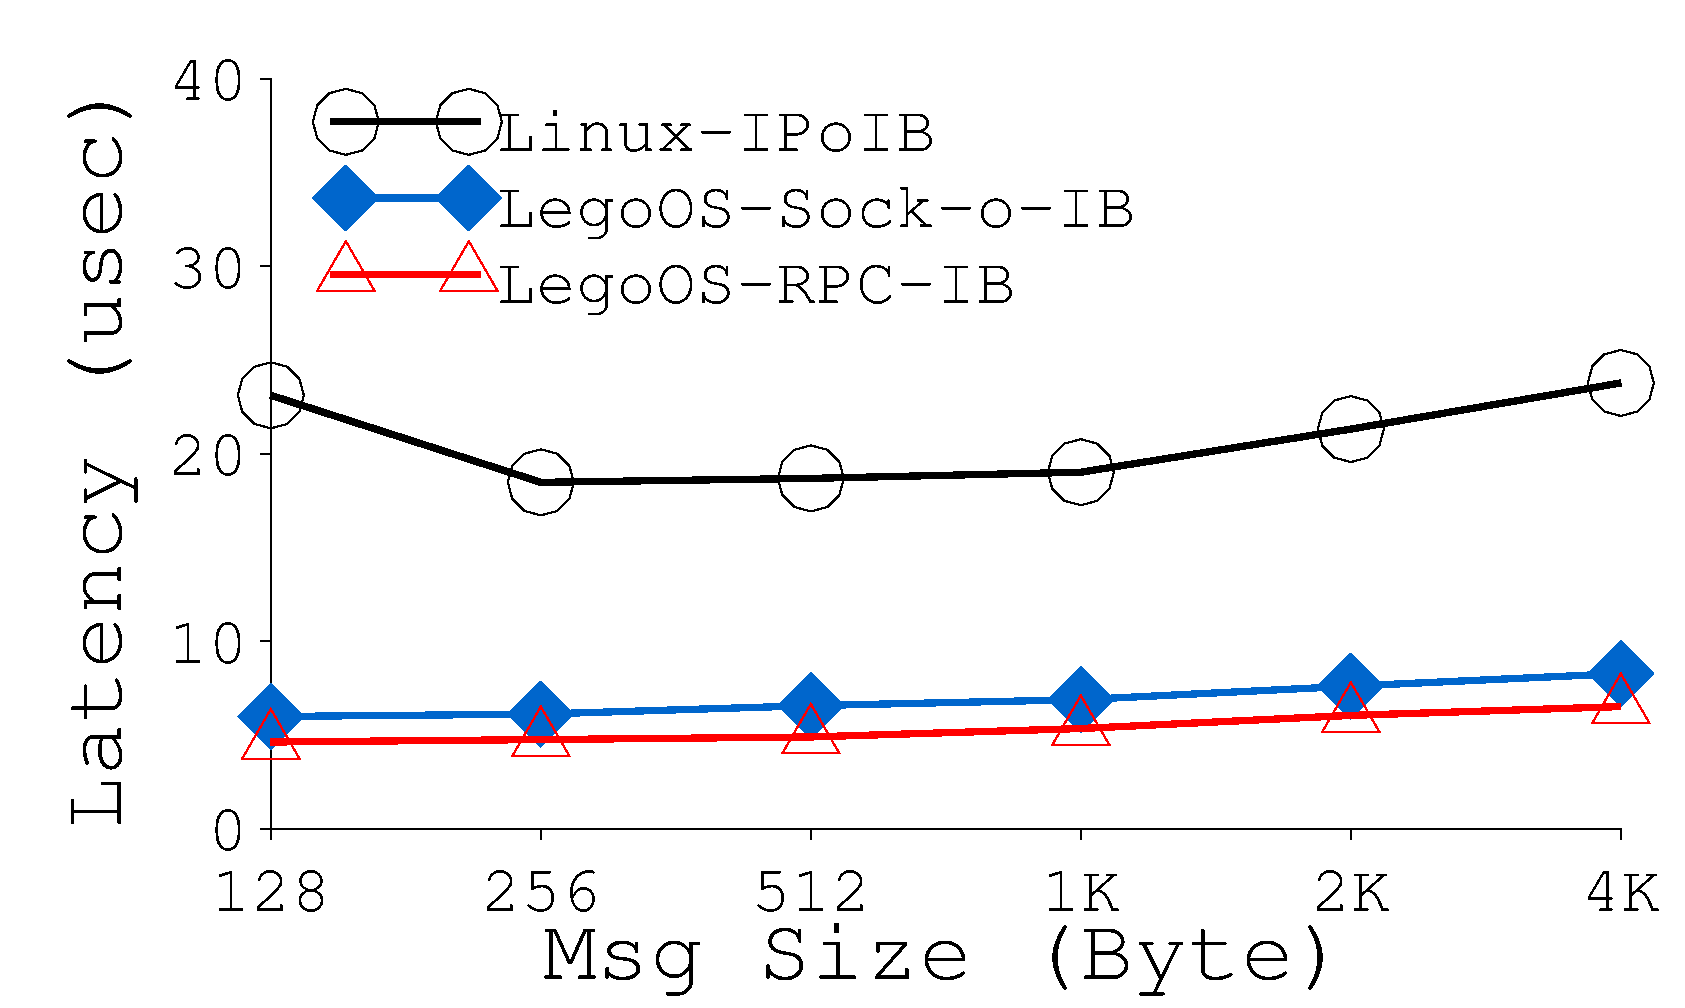
\includegraphics[width=0.5\textwidth]{lego/Figures/g_plot_LEGO_latency.pdf}}
\caption[Network Latency.]{Network Latency.}
\label{fig-net-latency}
\end{center}
\end{figure*}
}
{
\begin{figure*}[th]
\begin{center}
\centerline{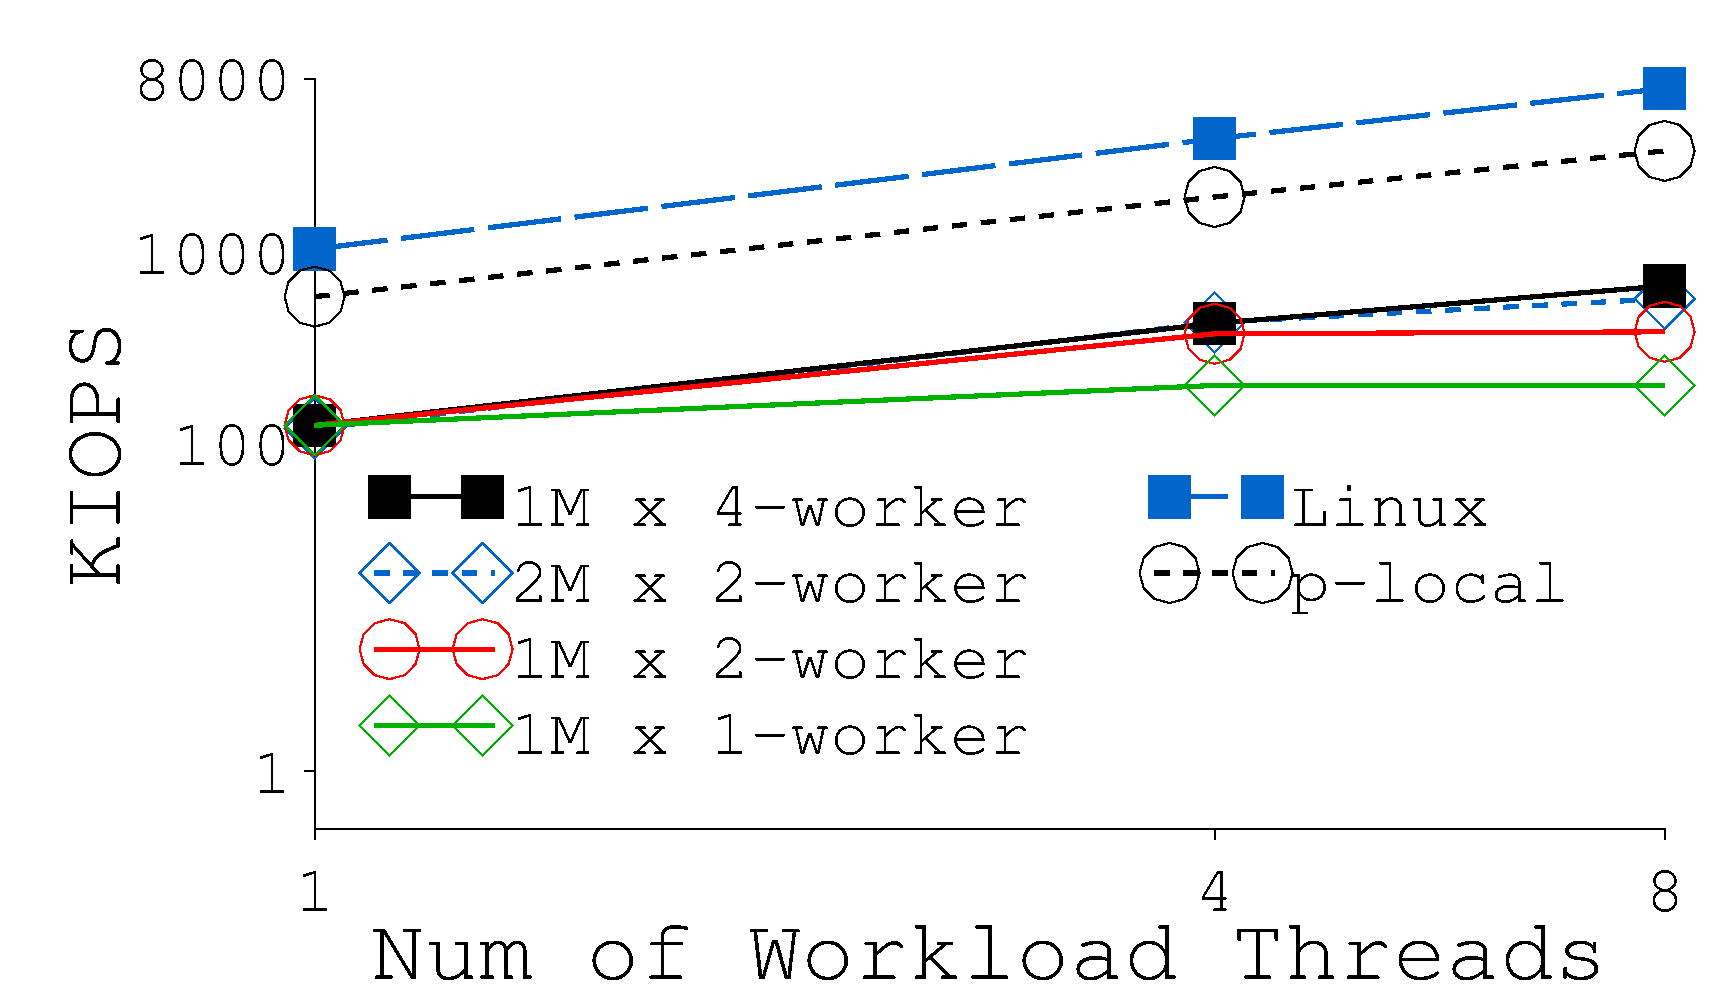
\includegraphics[width=0.5\textwidth]{lego/Figures/g_plot_LEGO_iops_memory.pdf}}
\caption[Memory Throughput]{Memory Throughput.}
\label{fig-iops-memory}
\end{center}
\end{figure*}
}
{
\begin{figure*}[th]
\begin{center}
\centerline{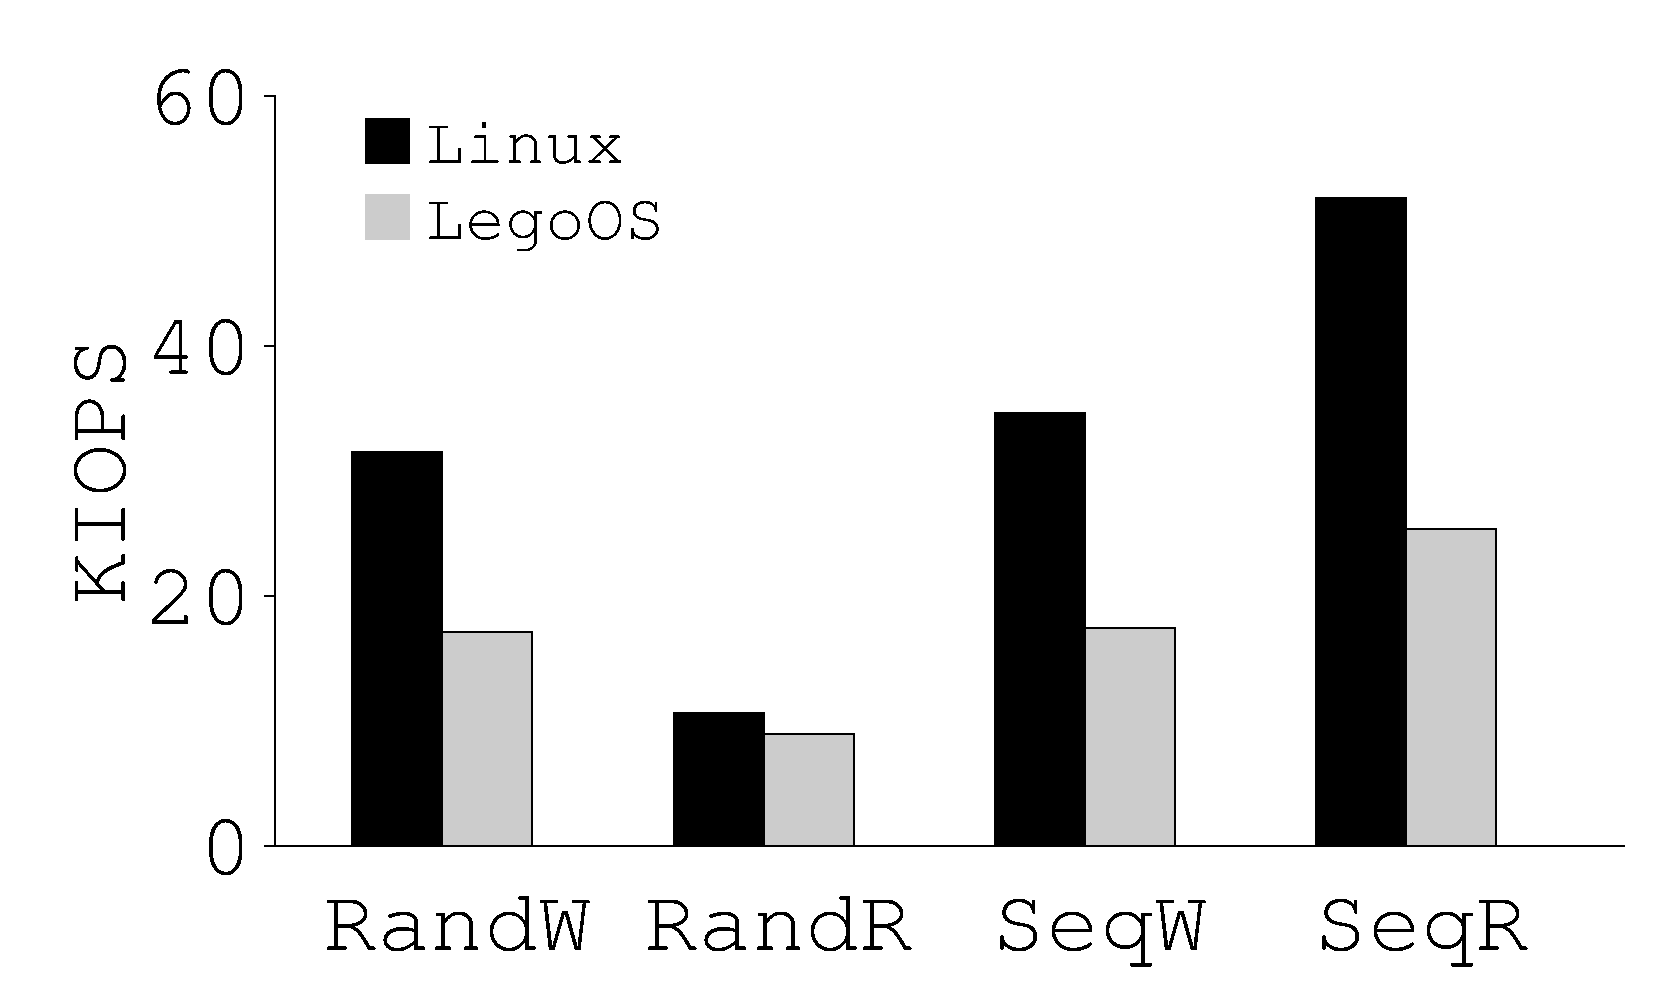
\includegraphics[width=0.5\textwidth]{lego/Figures/g_plot_LEGO_iops_storage.pdf}}
\caption[Storage Throughput.]{Storage Throughput.} 
\label{fig-iops-storage}
\end{center}
\end{figure*}
}
{
\begin{figure*}[th]
\begin{center}
\centerline{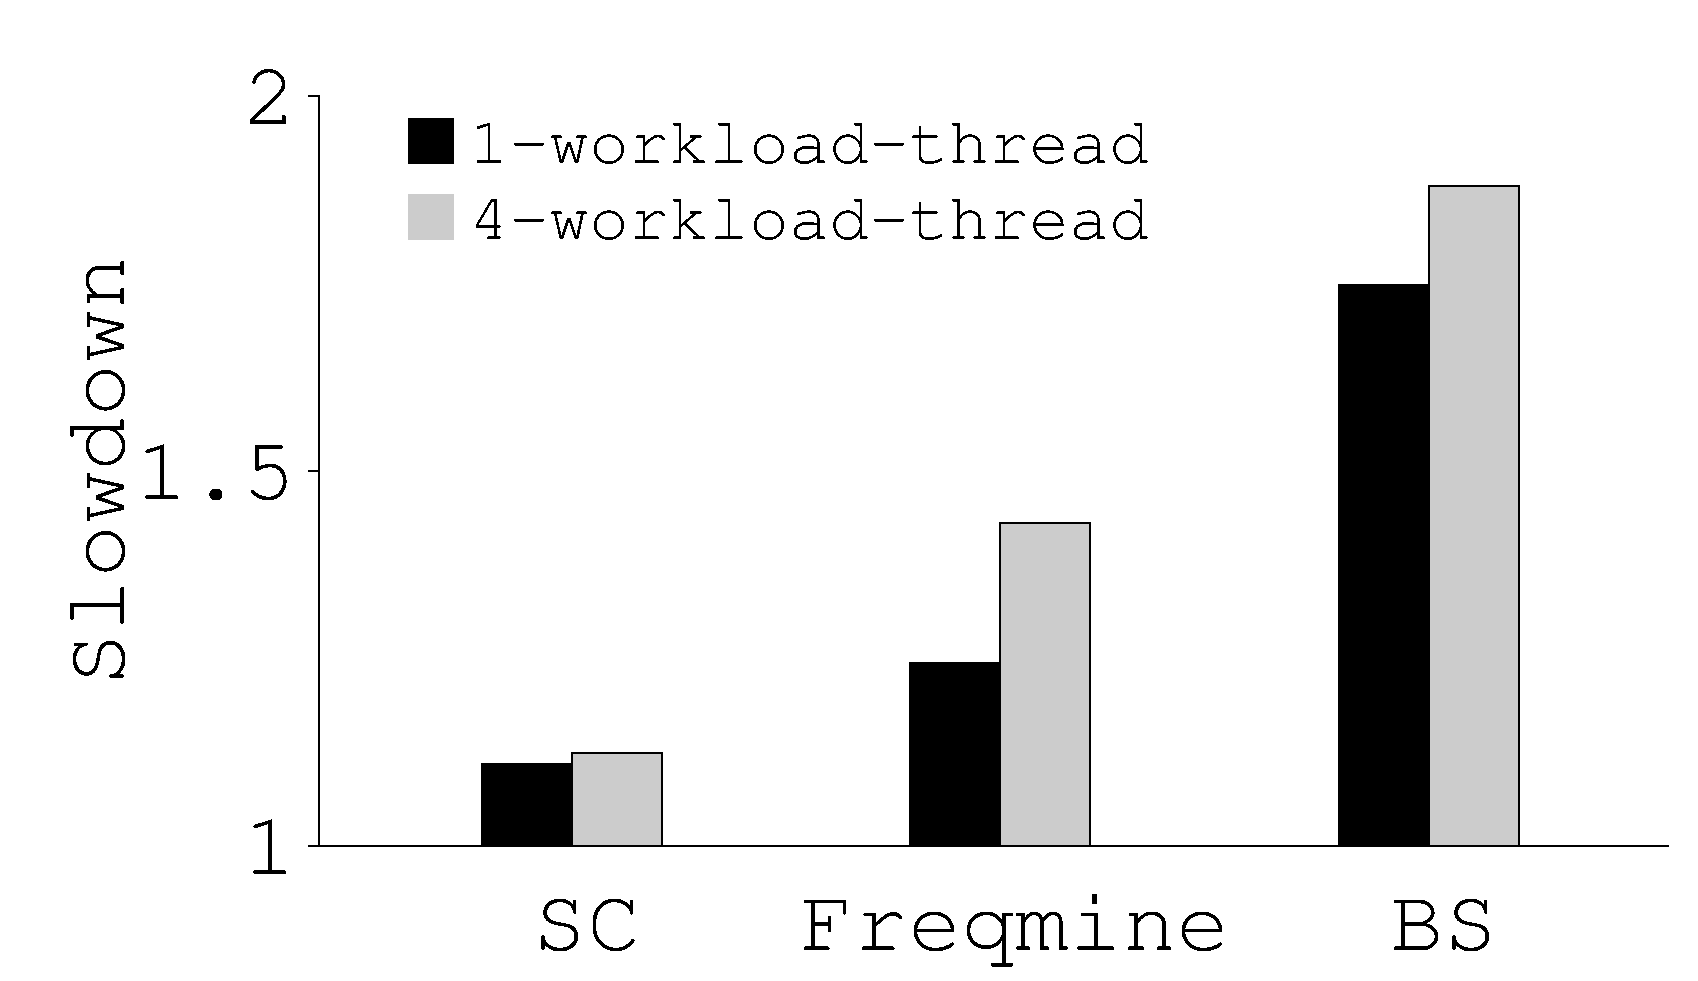
\includegraphics[width=0.5\textwidth]{lego/Figures/g_plot_LEGO_parsec.pdf}}
\caption[PARSEC Results.]{PARSEC Results. SC: StreamClsuter. BS: BlackScholes.}
\label{fig-parsec}
\end{center}
\end{figure*}
}
{
\begin{figure*}[t]
\begin{center}
\centerline{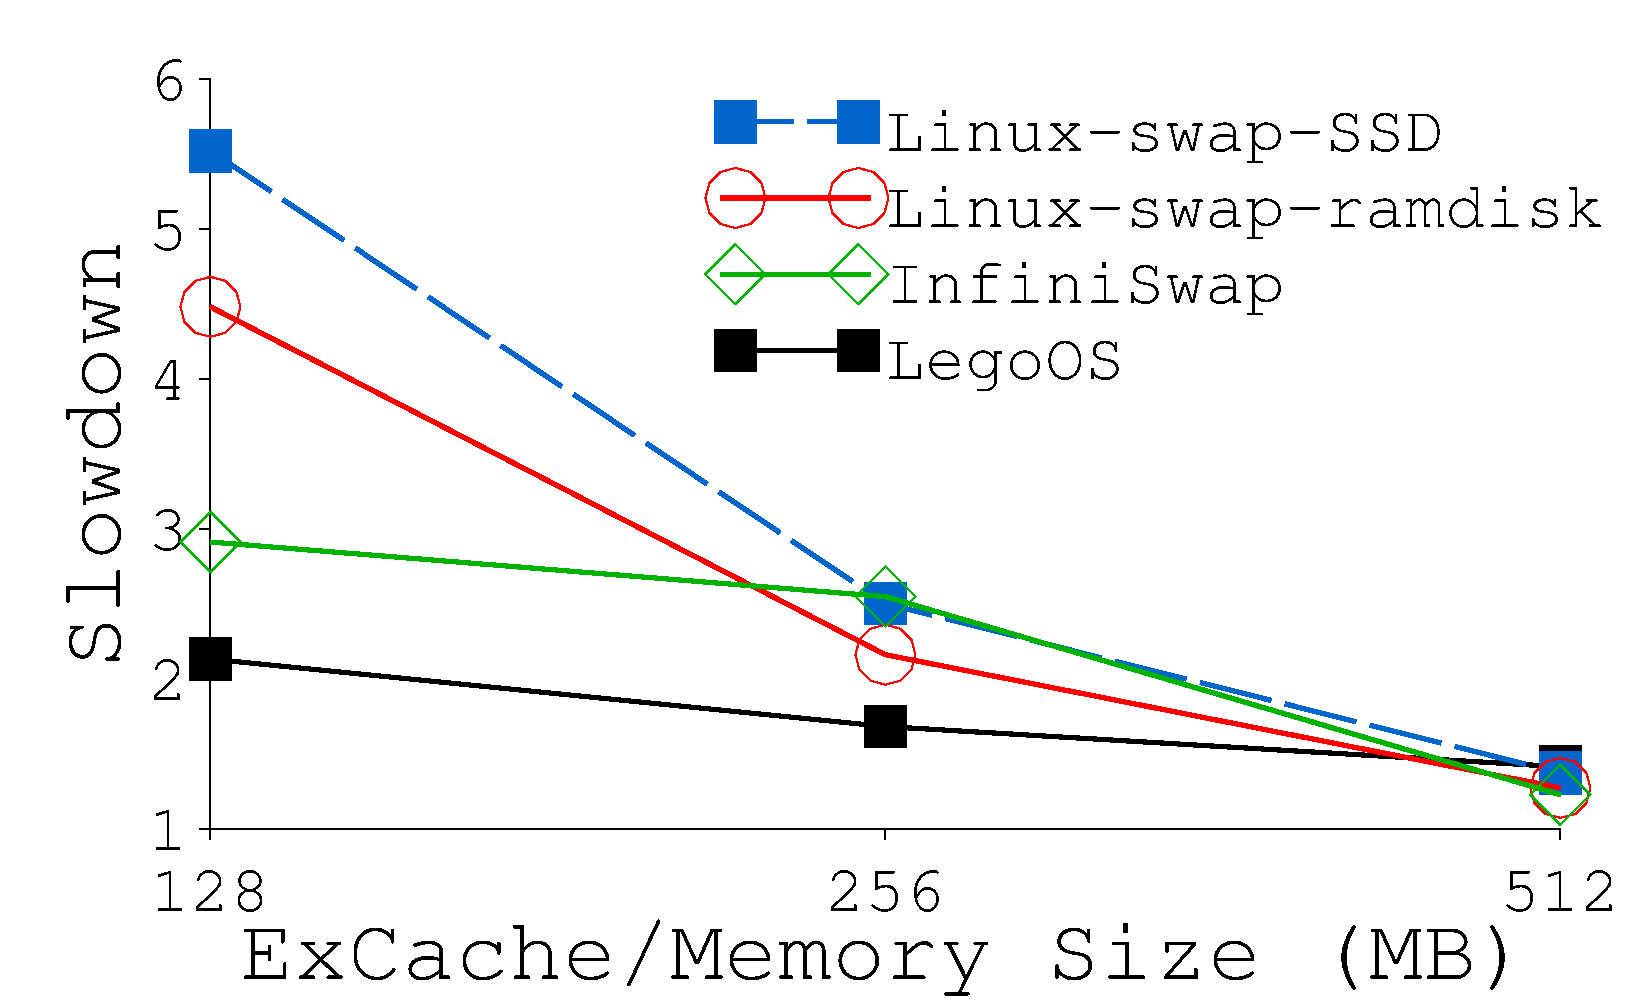
\includegraphics[width=0.5\textwidth]{lego/Figures/g_plot_LEGO_tf4.pdf}}
\caption[TensorFlow Performance.]{TensorFlow Performance.}
\label{fig-tf4}
\end{center}
\end{figure*}
}
{
\begin{figure*}[th]
\begin{center}
\centerline{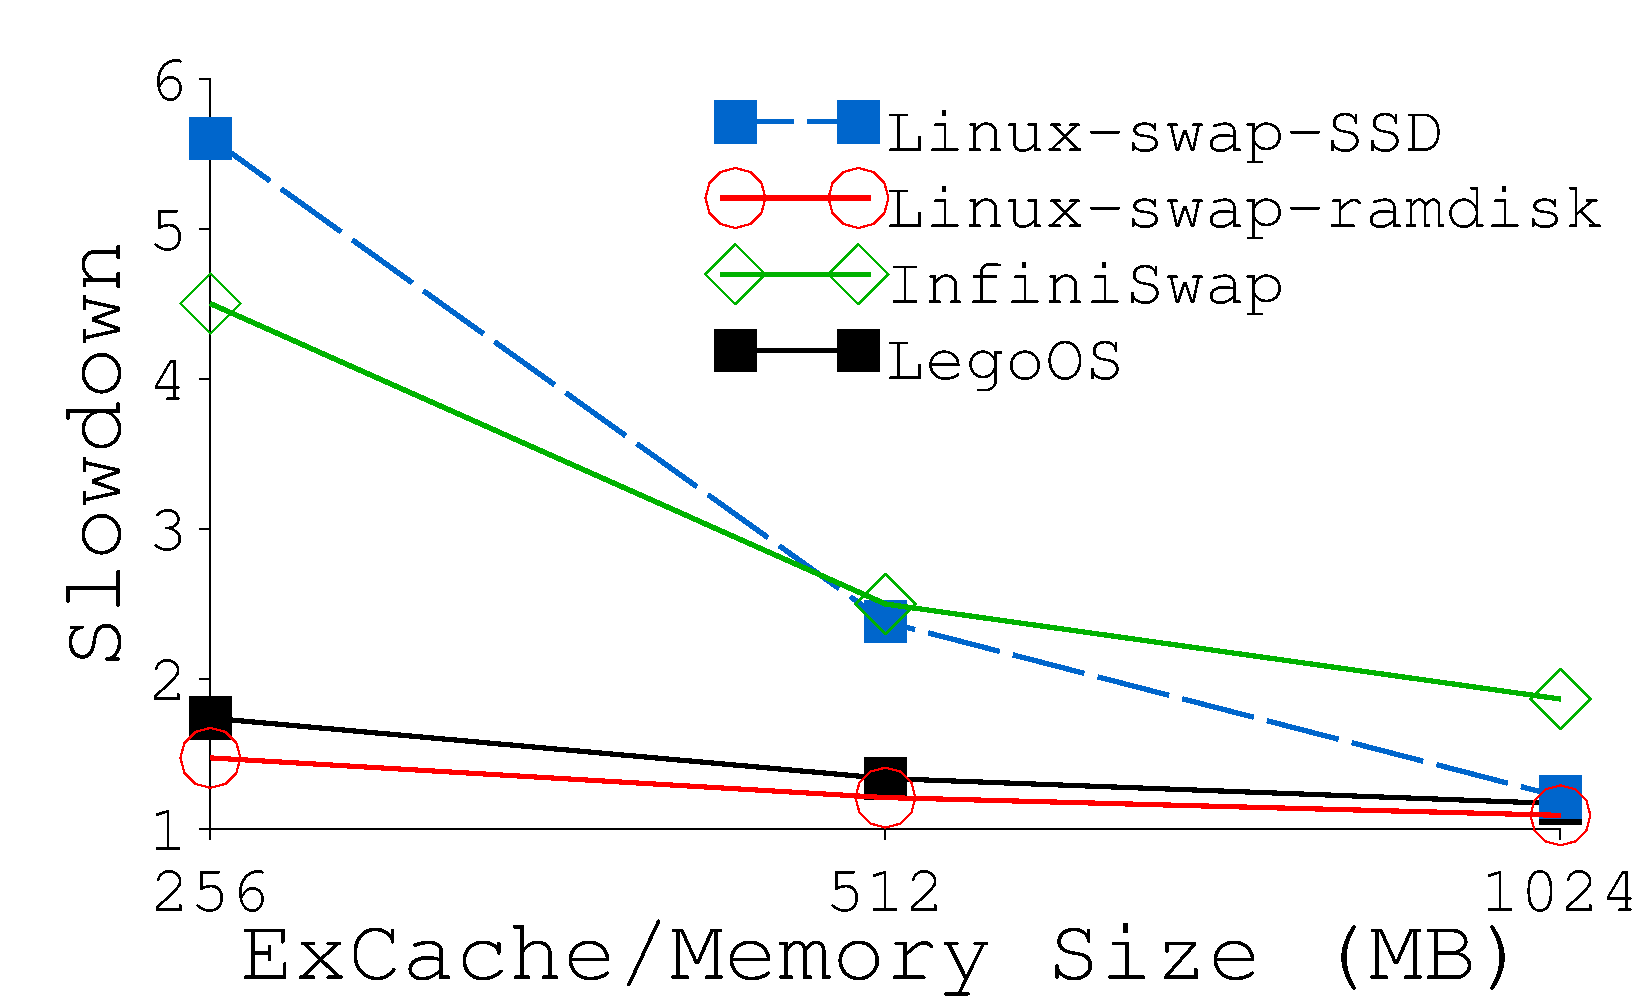
\includegraphics[width=0.5\textwidth]{lego/Figures/g_plot_LEGO_phoenix.pdf}}
\caption{Phoenix Performance.}{Phoenix Performance.}
\label{fig-phoenix}
\end{center}
\end{figure*}
}
{
\begin{figure*}[th]
\begin{center}
\centerline{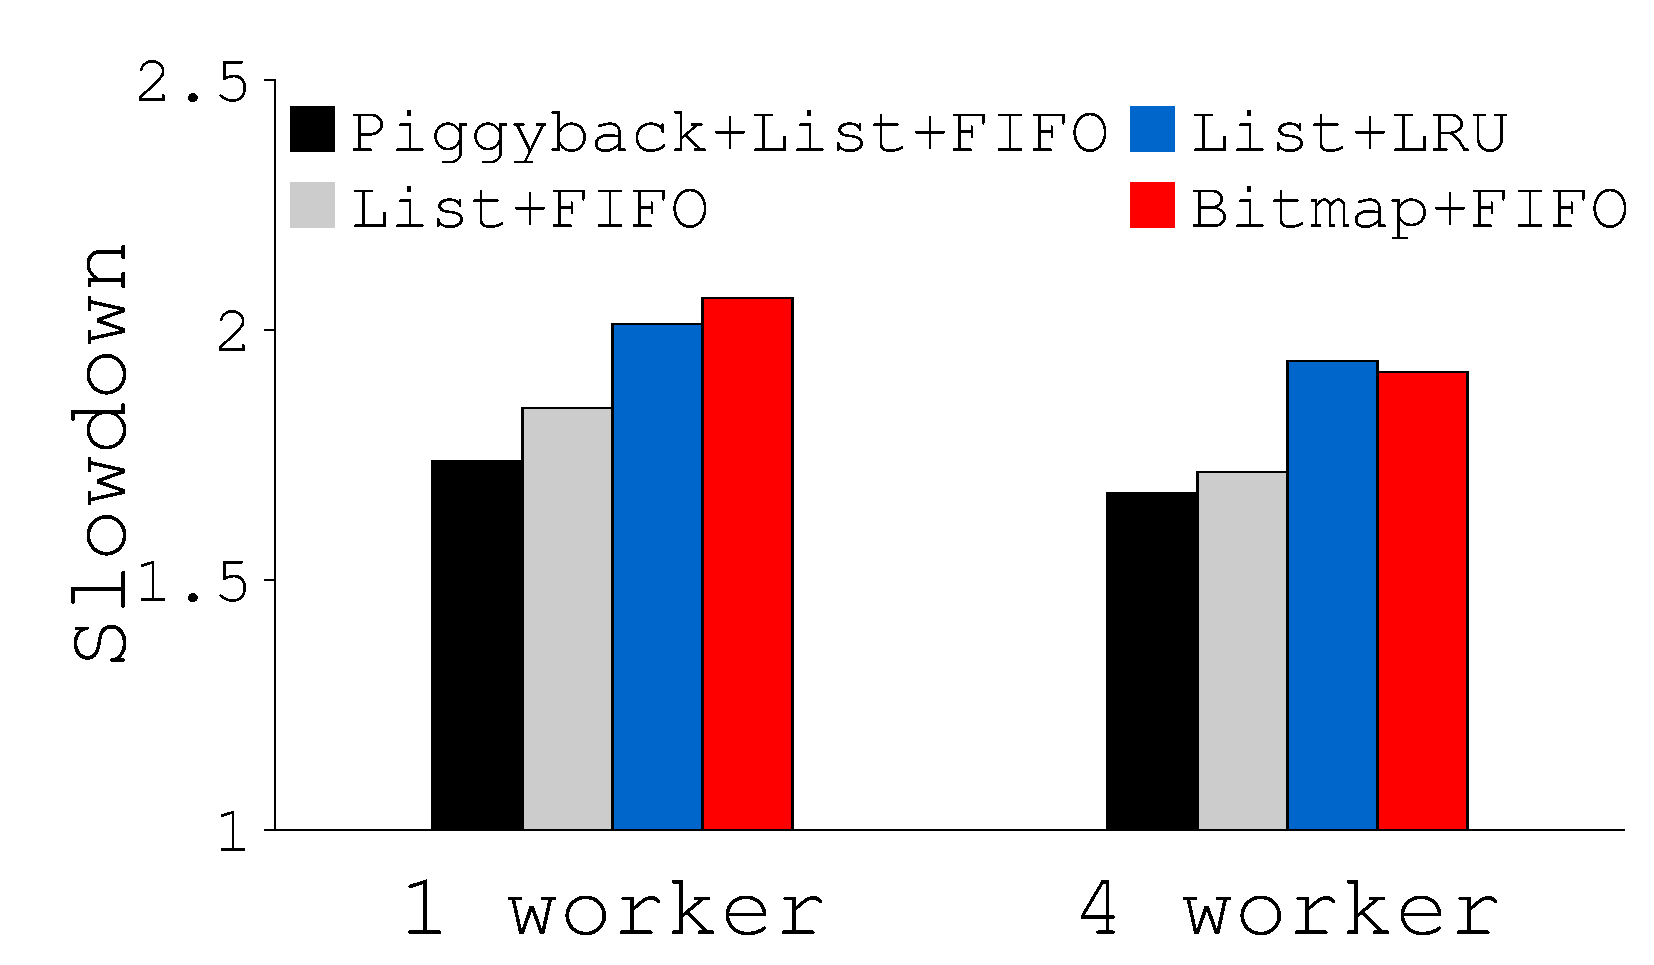
\includegraphics[width=0.5\textwidth]{lego/Figures/g_plot_LEGO_excache_tech.pdf}}
\caption{ExCache Management.}{ExCache Management.}
\label{fig-excache-opt}
\end{center}
\end{figure*}
}
{
\begin{figure*}[th]
\begin{center}
\centerline{\includegraphics[width=0.5\textwidth]{lego/Figures/g_plot_LEGO_number_memory_rep.pdf}}
\caption[Memory Config.]{Memory Config.}
\label{fig-mem-rep}
\end{center}
\end{figure*}
}
%{
\begin{figure}[th]
\begin{minipage}{0.01in}
\end{minipage}
\begin{minipage}{0.66\columnwidth}
\begin{center}
\centerline{\includegraphics[width=1.0\columnwidth]{Figures/g_plot_LEGO_number_memory_rep.pdf}}
\vspace{-0.1in}
\mycaption{fig-mem-rep}{\small{Memory Config.}}
{
%The effect of having multiple memory components and memory replication.
}
\end{center}
\end{minipage}
\vspace{-0.15in}
\end{figure}
}

\section{Evaluation}
\label{sec:results}

This section presents the performance evaluation of \lego\ using micro- and macro-benchmarks and two unmodified real applications.
We also quantitatively analyze the resource packing and failure rate of \lego.
We ran all experiments on a cluster of 10 machines, each with two Intel Xeon CPU E5-2620 2.40GHz
processors, 128 GB DRAM, and one 40 Gbps Mellanox ConnectX-3 InfiniBand network adapter;
a Mellanox 40 Gbps InfiniBand switch connects all of the machines. 

\subsection{Micro- and Macro-benchmark Results}
\noindent{\textit{\uline{Network performance.}}}
Network communication is at the core of \lego's performance.
Thus, we evaluate \lego's network performance first before evaluating \lego\ as a whole.
Figure~\ref{fig-net-latency} plots the average latency of sending messages with socket-over-InfiniBand (IPoIB) in Linux,
\lego's implementation of socket on top of InfiniBand (Lego-Sock-o-IB), and \lego's implementation of RPC over InfiniBand (Lego-RPC-IB).
\lego\ use Lego-RPC-IB for all its internal network communication across components and use Lego-Sock-o-IB for 
all application-initiated socket network requests.
Both \lego's networking stacks significantly outperform Linux's.
%which partially explain why \lego\ outperforms nbdX in \S\ref{sec:appresults}.

\noindent{\textit{\uline{Memory performance.}}}
To measure the raw performance of \mcomponent, we ran a multi-threaded user-level micro-benchmark 
where each thread performs one million sequential 4\KB\ memory load in a heap.
We use a huge, empty \excache\ (32\GB) to run this test, 
so that each memory access can generate an \excache\ (cold) miss and go to the \mcomponent.
Figure~\ref{fig-iops-memory} compares \lego' \mcomponent\ performance 
with Linux's single-node memory performance using this workload.
We vary the number of \mcomponent\ worker threads from 1 to 8 (only showing 1, 2, 4 in the figure)
and found that using more \mcomponent\ worker threads improves throughput when an application has high parallelism,
but using 4 worker threads can already saturate the performance.
We also evaluated the optimization technique in \S~\ref{sec:zerofill} (p-local in the figure).
As expected, bypassing \mcomponent\ with this \pcomponent-local lines significantly 
improves memory access performance.
The difference between p-local and Linux demonstrates the overhead of trapping to kernel and setting up \excache\ in our emulation.
\if 0
A single user thread has maximum 125 KIOPS.
Multi-threads' throughput is limited the number of \mcomponent's workers.
4 workers threads can achieve 668 KIOPS while running 8 threads. This
suggests \lego's \excache\ and \mcomponent\ scales well.
We also evaluated ~\ref{sec:zerofill}'s optimization on memory access, labeled
as Zerofill. This optimization greatly improved memory access throughput: each
thread can achieve 587 KIOPS. Zerofill is still slower than Linux because we
have the extra overhead to setup \excache.
%\lego's memory throughput scales well with the number of workload threads and achieves
%comparable performance even all \excache\ misses are across the network. 
\fi

\noindent{\textit{\uline{Storage performance.}}}
To measure the performance of \lego's storage system, we ran a single-thread micro-benchmark 
that performs random 4\KB\ read/write to a 25\GB\ file on an Samsung PM1725s NVMe SSD (the total amount of data accessed is 1\GB).
For write workloads, we issues an {\em fsync} after each {\em write} to test the performance of writing all the way to the SSD.
Figure~\ref{fig-iops-storage} presents the throughput of this workload when running on \lego\ and on single-node Linux.
For \lego, we use one \mcomponent\ to store the buffer cache of this file and initialize the buffer cache to empty
so that file I/Os can go to the storage layer (Linux also uses an empty buffer cache).
Our results show that Linux's performance is determined by the SSD's read/write bandwidth.
\lego's read performance is close to Linux, since network cost is relatively low compared to the SSD's read performance.
With better SSD write performance, network cost has a higher impact.
\lego's write-and-fsync performance is worse than Linux because
\lego\ requires one RTT between \pcomponent\ and \mcomponent\ to perform write 
and two RTTs (\pcomponent\ to \mcomponent, \mcomponent\ to \scomponent) for fsync.

\noindent{\textit{\uline{PARSEC results.}}}
We evaluated \lego\ with a set of workloads from the PARSEC benchmark suite~\cite{PARSEC},
including Blackscholes, FreqMine, StreamCluster, Swaptions, and x264.
These workloads are a good representative of compute-intensive datacenter applications, 
ranging from machine-learning algorithms to streaming processing ones.
Figure~\ref{fig-parsec} presents the slowdown of \lego\ 
over single-node Linux with enough memory.
\lego\ uses a fixed \excache\ size of 128\MB\ for these tests and 1, 2, and 4 \mcomponent s.
The two streaming workloads, StreamCluster and x264, perform the best because of their 
memory access pattern in batches (each batch around 95\MB\ to 110\MB).
Blackscholes and Freqmine have a larger resident memory size of around 630\MB.
This result suggest that stream processing is a good fit to \lego.
Finally, for these PARSEC workloads, the number of \mcomponent s have no or small effects.

\if 0
\noindent{\textit{\uline{Filebench results.}}}
\fixme{TODO. We are working on getting Filebench results with its varmail, fileserver, and webserver workloads.}
\fi

\subsection{Application Performance}
\label{sec:appresults}
We evaluated \lego's performance with two real, unmodified applications, 
TensorFlow~\cite{TensorFlow} and Phoenix~\cite{Ranger07-HPCA}, a single-node multi-threaded implementation of MapReduce~\cite{DeanEtAl04-MapReduce}.
TensorFlow's experiments use the Cifar-10 dataset~\cite{CIFAR-DS} and Phoenix's use a Wikipedia dataset~\cite{Wiki-DS}.
Unless otherwise stated, the base configuration used for all TensorFlow experiments
is 256\MB\ 64-way \excache, one \pcomponent, one \mcomponent, and one \scomponent.
The base configuration for Phoenix is the same as TensorFlow's with the exception that the base \excache\ size is 512\MB,
The total amount of virtual memory addresses touched in TensorFlow is 2.7\GB\ and 1.75\GB\ for Phoenix.
The total resident memory (minimal amount of memory needed to run an application without swapping) 
for TensorFlow and Phoenix is 0.9\GB\ and 1.7\GB.
Our default \excache\ sizes are set as roughly 25\% of total resident memory.
We ran both application with four threads.

\noindent{\textit{\uline{\excache\ size.}}}
Figures~\ref{fig-tf4}, and \ref{fig-phoenix} plot the TensorFlow and Phoenix run time comparison across 
\lego, two remote paging systems (InfiniSwap~\cite{GU17-NSDI} and Mellanox nbdX~\cite{nbdX}), 
single-node Linux (v4.9.47) with a swap file in a local high-end NVMe SSD, and Linux with a swap file in local ramdisk.
All values are calculated as a slowdown to running the applications on a single-node Linux that have enough local resources (main memory, CPU cores, and SSD).
For systems other than \lego, we change the main memory size to the same size of \excache\ in \lego, with rest of the memory on swap file. 
With roughly 25\% resident memory, the overhead of TensorFlow, and Phoenix on \lego\ are 
71\%, and 52\%\ compared with monolithic Linux that has all the memory needed for the workload.
%\yizhou{But for multi-threaded TF, we saw a 3.5x slowdown. The reason is simple: with multiple threads,
%the program execution becomes much faster, which leads to higher rate of ExCache conflicts.}
%\fixme{How to explain the difference between TF-4 and Phoenix? They are both 4 threads. The explanation is not convincing.}

\lego's performance is significantly better than swapping to SSD and to remote memory 
largely because of our efficiently-implemented network stack, simplified code path compared with Linux paging subsystem,
and the optimization technique proposed in \S\ref{sec:zerofill}.
Surprisingly, it is similar or even better than swapping to local memory, even when \lego's memory accesses are across network.
This is mainly because ramdisk goes through buffer cache and incurs memory copies between the buffer cache and the in-memory swap file.
%because ramdisk 
%We suspect this is due to the overhead in ramdisk.
%As expected, with less main memory and with smaller \excache, Linux and \lego's performances both decrease.

\if 0
Comparing TensorFlow with Phoenix, \lego\ works better with TensorFlow.
This is because TensorFlow has a repeating pattern of memory accesses during its computation.
It first loads the whole dataset into memory. 
Afterwards, it performs computation on a rotating {\em batch\_size} of in-memory data (\eg, 100 images).
This pattern fits well with \lego's memory model: a small set of memory with frequent accesses and a large amount of total memory.
\fi

\lego's performance results are not easy to achieve and we went through rounds of design and implementation refinement.
Our network stack and RPC optimizations yield a total improvement of up to 50\%.
For example, we made all RPC server (\mcomponent's) replies {\em unsignaled} to save \mcomponent' processing time
and to increase its request handling throughput.
Another optimization we did is to piggy-back dirty cache line flush and cache miss fill into one RPC.
The optimization of first anonymous memory access (\S\ref{sec:zerofill}) improves \lego's performance further by up to 5\%.

\noindent{\textit{\uline{\excache\ Management.}}}
Apart from \excache\ size, how it is managed can also largely affect application performance.
We first evaluated factors that could affect \excache\ hit rate and found that higher associativity improves hit rate
but the effect diminishes when going beyond 512-way.

We then focus on evaluating the miss cost of \excache, since the miss path is handled by \lego\ in our design.
We compare the two eviction policies supported in \lego: FIFO and LRU,
and two implementations of finding an empty line in an \excache\ set: linearly scan a free bitmap
and fetching the head of a free list.
Figure~\ref{fig-excache-opt} presents these comparisons with 1 and 4 \mcomponent\ worker threads. 
All tests use TensorFlow's default setting (256\MB\ 64-way \excache).
Using bitmaps for this \excache\ configuration is always worse than using free lists
because of the cost to linearly scan a whole bitmap,
and bitmaps perform even worse with higher associativity.
%When associativity is high, using bitmap incurs large overhead, while free list's operation has constant delay.
Surprisingly, FIFO performs better than LRU in our tests, even when LRU utilizes access locality pattern.
We attributed LRU's worse performance to the lock contention it incurs;
the kernel background thread sweeping the \excache\ locks an LRU list when adjusting the position of an entry in it,
while \excache\ miss handler thread also needs to lock the LRU list to grab its head.
%\excache\ has two eviction policy: FIFO and LRU. LRU has a kernel background thread dynamically
%adjust \excache\ line. The adjustment will pollute cache and content lock.
%LRU has extra 17\% slowdown compared with FIFO, when using free list based \excache.
%While both use FIFO, bitmap is 22\% slower than free list.
%A \excache\ using free list and FIFO eviction policy is the best configuration.
%Next, we vary the number of \mcomponent's worker threads. From 1 to 4 worker threads, we see a reduction
%of 13\% for List+FIFO.

%{
\begin{table*}[th]\footnotesize
\begin{center}
\begin{tabular}{ l | c | c | c | c | c | c | c | c | c }
\small OS & \small Res. Dis. & \small Hetero & \small Elastic & \small Limited h/w & \small Distributed & \small Failure & \small Msging & \small Linux ABI & \small Abstraction \\
\hline
\lego\ & \cmark & \cmark & \cmark & \cmark & \cmark & \cmark & \cmark & \cmark & Dist \\
Linux & \xmark & \xmark & \xmark & \xmark & \xmark & \xmark & \xmark & \cmark & Single \\
Barrelfish & \xmark & \cmark & \cmark & \xmark & \xmark & \xmark & \cmark & \xmark & Single\\
Helios & \xmark & \cmark & \xmark & \cmark & \xmark & \xmark ? & \cmark & \xmark & Single \\
fos & \xmark & \cmark & \cmark & \xmark & \cmark & \xmark & \cmark & \xmark & Single \\
Amoeba & \cmark\ * & \xmark & \cmark & ? & \cmark & \cmark & \cmark & \xmark & Single\\ 
Sprite & \xmark & \xmark & \xmark & \xmark & \cmark & \cmark &  & \xmark & Single \\
L4 & \xmark & & & \xmark & \xmark & & & \xmark & Single \\
Corey & \xmark & & & \xmark & \xmark & & \cmark & \xmark & Single \\
Hive & \xmark & ? & ? & \xmark & \cmark ? & \cmark & \xmark & \xmark & Single \\
\end{tabular}
\end{center}
\vspace{-0.1in}
\mycaption{tbl-os-comp}{\lego\ Comparison to Related OSes.}
{
Comparison in the support for resource disaggregation, hetereogeneity, elastiticy 
designing with hardware constraints, handling distributed nature, handling failure, 
support for unmodified Linux ABI, and whether it appears as a distributed set of nodes 
or a single OS image.
* Amoeba manages pool of resources.
}
%\vspace{-0.1in}
\end{table*}
}

\noindent{\textit{\uline{Number of \mcomponent s and replication.}}}
Finally, we study the effect of number of \mcomponent s and memory replication.
Figure~\ref{fig-mem-rep} plots the performance slowdown as the number of \mcomponent s increases from one to four.
Using more \mcomponent s improves performance by up to 3\%.
A main reason why the improvement is small and unstable is because these applications perform
most memory allocation in the beginning of their run.
At that time, \lego\ allocates \vregion\ owners with limited information in memory access load.
Migrating allocated data across \mcomponent s can potentially solve this problem,
an improvement we leave for future.
%We currently do not support memory migration and leave it as a planned future work.

We also evaluated \lego's memory replication in Figure~\ref{fig-mem-rep}.
Overall, our best-effort replication mechanism is almost free in performance (0.1\% to 1\%) and in space (a static 1\MB\ overhead).
We also tested synchronous replication where foreground waits for the write back of backup memory log.
The synchronous replication scheme has an overhead of 1.2\%.

{
\begin{table*}[th]\footnotesize
\begin{center}
\begin{tabular}{ l || c | c | c | c | c | c || c | c}
 & Processor & Disk & Memory  & NIC & Power & Other & Monolithic & \lego\ \\
\hline
%Unit Cost & \$6500 & \$530 & \$760 & \$360 & \$380 &\$320 & \$7400 & N/A \\
%Monolithic & 100 & (200) & (400) & (100) & (100) & 100 & 3  & \$704,200\\
%Disaggregation & 0 & 100 & 200 + 50 & 0 & 100 & 125 & 4 & \$350,600 \\

MTTF (year) & 204.3 & 33.1 & 289.9 & 538.8 & 100.5 & 27.4 & 5.8 & 6.8 - 8.7 \\
%MTTF  & &&&&&& \\

\end{tabular}
\end{center}
\vspace{-0.2in}
\mycaption{tbl-failure}{Mean Time To Failure Analysis.}
{
MTTF numbers of devices (columns 2 to 7) are obtained from~\cite{Failure-Disk-FAST07}
and MTTF values of monolithic server and \lego\ are calculated using the per-device MTTF numbers.
%Unit: year.
%MTTPF: Mean Time To Permanent (hardware) Failure, MTTF: Mean Time To (all types of hardware) Failure.
%Per-device MTTF used to calculate MTTPF are collected from Table 3 in \cite{Failure-Disk-FAST07}.
%Processor failure includes the failure of CPU, fan, and CPU heat sink (for both monolithic server and Lego).
}
%\vspace{-0.1in}
\end{table*}
%\vspace{-0.1in}
}




\if 0
We now present the results of how \excache\ configuration affects application performance.
Figure~\ref{fig-associativity} plots the performance slowdown and number of \excache\ misses as \excache\ associativity increases.
With higher associativity (\ie, each \excache\ set is bigger), the performance of TensorFlow improves slowly,
but surprisingly, the performance of Phoenix drops.
To understand the cause, we collected the number of \excache\ misses. 
TensorFlow's misses drop as associativity increases, 
while Phoenix's misses stay similar across different associativity.
We found our LRU-list implementation is a major reason why performance decreases as \excache\ associativity increases and \excache\ misses stay the same.
We use a per-set LRU list and lock it when inserting, deleting, and adjusting a \excache\ line's metadata entry in the list.
With multiple threads contending for a set, the locking overhead increases as a set becomes bigger.
We plan to solve this problem by changing the per-set LRU list to a per-core and per-set list in the future.
\fi
%which we suspect is because it evenly distribute accesses within its working sets.
%1) the workloads we tested are not sensitive to set associativity mostly because their wss are evenly distributed (which is not a bad thing, cos with small associativity the cost of tag comparison is lower), 2) with higher associativity we pay a higher lock contention overhead, something we can improve by changing to per-core LRU list, for future work

\subsection{Resource Packing}
\label{sec:cost}
To analyze how multiple applications run on \lego\ and how \lego\ allocates resources for them,
we use a simple scenario of running one TensorFlow instance and two Phoenix instances together in three settings:
1) run each instance separately on a monolithic Linux machine with 8 cores and 2\GB\ memory (three machines in total);
2) run one TensorFlow and one Phoenix on one Linux machine of the same type and 
run one Phoenix on a second Linux machine of the same type;
%2) run all three instances together on one Linux machine of the above type;
3) run the three instances on two \lego\ processors (each with 8 cores) and two \lego\ \mcomponent s (each with 2\GB\ memory).
The resident memory of a TensorFlow instance is around 0.5\GB\ and that of Phoenix is around 1.7\GB.

In the first setting, all three instances have enough memory and will not trigger any swap. 
We use the performance of TensorFlow and Phoenix in this setting (\ie, each running on a single-node Linux with enough resources)
as the baseline of performance comparison.
This setting achieves the best performance but it comes with the cost of high memory resource waste (2.1/6 = 35\%),
and it requires three full machines.
The second setting uses two Linux machines. 
The first machine's memory is fully utilized while 1.7\GB\ memory on the second machine is utilized, yielding a total of 7.5\% resource waste.
Running one TensorFlow and one Phoenix on the first machine results in memory swap (total resident memory is 2.2\GB, which exceeds the 2\GB\ main memory size),
slowing down TensorFlow's performance by 27\% and Phoenix's performance by 31\%).

With the third setting of a \lego\ cluster, \lego's GPM and GMM dynamically allocates CPU cores and memory to 
the three running instances. 
Since \lego\ does not split a process across processors, one TensorFlow process and one Phoenix process
run on one processor, and the other Phoenix process runs on a second processor.
The memory of these three processes are spread across the two \mcomponent s,
resulting in total memory utilization of 3.9/4 = 98\% without any memory swapping.
The TensorFlow and Phoenix that run together on the first processor incur run time slowdown of 
5.9\x\ and 1.8\x, while the Phoenix that runs alone on the second processor has a slowdown of 1.5\x.
\fixme{still trying to get better results for the co-running TensorFlow and Phoenix.}

This experiment demonstrates \lego's advantages in efficient resource packing.
\lego\ can allocate memory from any \mcomponent\ regardless of where a process runs at.
In contrast, monolithic OSes like Linux have to allocate memory from the same machine where
a running process is at, resulting in either high memory wastes or performance overhead due to memory swapping.

\if 0
Before presenting \lego's performance results, we first discuss the estimated monetary cost of 
\lego's hardware system and how it compares with monolithic servers.
Table~\ref{tbl-cost} summarizes the market price of a packaged monolithic server 
with similar configuration as the servers we use in our experiments (see above)
and the price of hardware devices in it. 
We list InfiniBand NIC and switch prices separately.
We also estimate the number of components a disaggregated cluster needs to provide the same 
resource as 100 monolithic servers.
We assume that without DIMM/channel bottleneck or other bus bottlenecks, 
each \mcomponent\ can host twice as much DRAM and every \scomponent\ can host two SSDs.

Overall, a disaggregated cluster costs only 50\% of a traditional server cluster.
With fewer CPU and DRAM, it will also significantly save energy cost.
We remind readers that our calculation here is only a rough estimation based on off-the-shelf market price
and on the results of CPU and memory being half utilized in current datacenters.
For example, we assume a 100\% resource utilization with a disaggregated cluster
and calculate the amount of CPU and DRAM it needs to be half of a regular cluster.
We also include a 25\% of disaggregated memory as processor-local \excache.
Although our calculation may not be accurate, but the conclusion and the trend are clear:
with better resource utilization, the total owning and operating costs of a disaggregated cluster is much lower than a monolithic server cluster. 
\fi

\subsection{Failure Analysis}
\label{sec:failure-results}
Finally, we provide a qualitative analysis on the failure rate of a \lego\ cluster compared to a monolithic server cluster.
Table~\ref{tbl-failure} summarizes our analysis.
We use two metrics to measure the failure rate of a cluster: 
1) Mean Time To Permanent (hardware) Failure (MTTPF), the mean time to the permanent failure of a server in a monolithic cluster
or a component in a \lego\ cluster;
2) Mean Time To Failure (MTTF), the mean time to all types of hardware failure (permanent and transient).
%that includes all failures that lead to machine outage, not only
%those that necessitate a hardware replacement.
MTTPF indicates the frequency of hardware replacement in a cluster, 
while MTTF implies application failures that are caused by hardware issues.
For MTTF, we further take into consideration the fault tolerance in a monolithic cluster and in \lego\ (\eg, redundant storage).

To calculate MTTPF (or MTTF) of a monolithic server, we first obtain the replacement frequency of different hardware devices in a server
(CPU, memory, disk, NIC, motherboard, case, power supply, fan, CPU heat sink, and other cables and connections)
from the real world (the COM1 and COM2 clusters in \cite{Failure-Disk-FAST07}).
For \lego, we envision every component to have a NIC and a power supply, 
and in addition, a \pcomponent\ to have CPU, fan, and heat sink, a \mcomponent\ to have memory, and a \scomponent\ to have a disk.
We further assume both a monolithic server and a \lego\ component to fail when any hardware devices in them fails
and the devices in them fail independently.
Thus, the MTTPF (or MTTF) can be calculated using the harmonic mean ({\em HM}) 
of the MTTPF (or MTTF) of each device.
% serial systems of components having
%independent exponentially distributed reliabilities.

\begin{equation}
MTTPF = \frac{HM_{i=0}^n(MTTPF_i)}{n}
\end{equation}

where $n$ includes all devices in a machine/component. MTTF is calculated similarly.

Further, when calculating MTTPF and MTTF of \lego, we estimate the amount of components needed in \lego\ 
to run the same applications as a monolithic cluster.
Our estimated worst case for \lego\ is to use the same amount of hardware devices 
(\ie, assuming same resource utilization as monolithic cluster).
\lego's best case is to achieve full resource utilization 
and thus requiring only about half of CPU and memory resources 
(since average CPU and memory resource utilization in monolithic server clusters is around 50\%~\cite{GoogleTrace,AliTrace}).

With better resource utilization and simplified hardware components (\eg, no motherboard),
\lego\ improves MTTPF by 17\% to 49\% compared to an equivalent monolithic server cluster.

\if 0
Best case:
\begin{equation}
MTTF_{Lego} = \frac{HM(MTTF_P, MTTF_M, MTTF_S)}{3}
\end{equation}

Worst case:
\begin{equation}
MTTF_{Lego} = \frac{HM(MTTF_P/2, MTTF_M/2, MTTF_S)}{3}
\end{equation}
\fi

\fixme{TODO: still need to find per-device MTTF numbers}.
\section{Related Work}
\label{sec:related}
%Below we contrast \lego\ to several related works.

%\boldparagraph{Resource Disaggregation.}
\paragraph{Hardware Resource Disaggregation.}
There have been a few hardware disaggregation proposals from academic and industry,
%break the traditional server-centric rack architecture into disaggregated resources.
including Firebox~\cite{FireBox-FASTKeynote}, HP "The Machine"~\cite{HP-TheMachine,HP-MemoryOS}, dRedBox~\cite{dRedBox-DATE},
and IBM Composable System~\cite{IBM-Composable}.
Among them, dRedBox and IBM Composable System package hardware resources in one big case 
and connect them with buses like PCIe.
The Machine's scale is a rack and it connects SoCs with NVMs with specialized coherent network.
FireBox is an early-stage project and is likely to use high-radix switches to connect  customized devices.
The disaggregated cluster we envision to run \lego\ on is one that hosts hundreds to thousands of
non-coherent, heterogeneous hardware devices, connected with a commodity network.
%Firebox~\cite{FireBox-FASTKeynote} is an ongoing project at Berkeley which aims to 
%use custom chips and new instruction set architecture to organize disaggregated racks.
%{\em The Machine} from HP~\cite{HP-TheMachine,HP-MemoryOS} is another ongoing project that builds racks with disaggregated resources and focuses on the usage of SoCs, persistent memory, and a memory-centric OS.
%These systems are at their early stage and do not provide or disclose software implementations.
%Moreover, they do not consider heterogeneity or failure issues in disaggregated cluster.
%\yizhou{check if they do handle failures.}
%We believe that we are the first to propose a distributed OS for resource disaggregation.
%are likely to adopt the resource pool architecture and 
%use simple high-radix fiber-optic or RDMA network to connect resource pools.
%Our proposed work decomposes racks further into independent resource components 
%and designs a new network layer for this architecture.

\paragraph{Memory Disaggregation and Remote memory.}
Lim \etal\ first proposed the concept of hardware disaggregated memory
with two models of disaggregated memory: using it as network swap device 
and transparently accessing it through memory instructions~\cite{Lim09-disaggregate,Lim12-HPCA}.
Their hardware models still use a monolithic server at the local side. 
\lego's hardware model separates processor and memory completely. %is different.

Another set of recent projects utilize remote memory without changing 
monolithic servers~\cite{Dragojevic14-FaRM,Nelson15-ATC,remote-region-atc18,GU17-NSDI,Novakovic16-SOCC,hotpot-socc17}.
For example, InfiniSwap~\cite{GU17-NSDI} transparently swaps local memory to remote memory via RDMA.
These remote memory systems help improve the memory resource packing in a cluster.
However, as discussed in \S\ref{sec:motivation}, unlike \lego, these solutions cannot solve other limitations 
of monolithic servers like the lack of hardware heterogeneity and elasticity. 

\paragraph{Storage Disaggregation.}
Cloud vendors usually provision storage at different physical machines\cite{deepview-nsdi18,url:aws-storage,url:vmware-vSAN}.
Remote access to hard disks is a common practice, because their high latency and low throughput
can easily hide network overhead~\cite{petal-asplos96,blizzard-nsdi14,Parallax-hotos15,Legtchenko-hotstorage17}.
While disaggregating high-performance flash is a more challenging task~\cite{FlashDisaggregation,url:facebook-lighting}.
Systems such as ReFlex~\cite{ReFlex}, Decibel~\cite{decibel-nsdi17}, and PolarFS~\cite{PolarFS-VLDB18},
tightly integrate network and storage layers to minimize software overhead in the face of fast hardware.
Although storage disaggregation is not our main focus now,
we believe those techniques can be realized in future \lego\ easily.


%\boldparagraph{Operating system design.}
%The concept of distributed operating systems dates back to early 90s. %late 80s and early 90s, with two OSes, Sprite and Amoeba.

\paragraph{Multi-Kernel and Multi-Instance OSes.}
Multi-kernel OSes like Barrelfish~\cite{Baumann-SOSP09,Barrelfish-DC}, Helios~\cite{Helios-SOSP}, Hive~\cite{Hive-SOSP}, and fos~\cite{fos-SOCC}
run a small kernel on each core or programmable device in a monolithic server,
and they use message passing to communicate across their internal kernels.
Similarly, multi-instance OSes like Popcorn~\cite{popcorn-eurosys15} and Pisces~\cite{Pisces-hpdc15} run multiple Linux kernel instances
on different cores in a machine. % to provide heterogeneous support and performance isolation.
Different from these OSes, \lego\ runs on and manages a distributed set of hardware devices;
it manages distributed hardware resources using a two-level approach and handles device failures (currently only \mcomponent).
In addition, \lego\ differs from these OSes in how it splits OS functionalities, where it executes the split kernels,
and how it performs message passing across components.
Different from multi-kernels' message passing mechanisms which are performed over buses or using shared memory in a server, 
\lego's message passing is performed using a customized RDMA-based RPC stack over InfiniBand or RoCE network.
Like \lego, fos separates OS functionalities and run them on different processor cores that share main memory.
Helios runs {\em satellite kernels} on heterogeneous cores and programmable NICs that are not cache-coherent.
% with the latter and non-coherent memory.
We took a step further by disseminating OS functionalities to run on individual, network-attached hardware devices. % and run split kernel at hardware controllers.
Moreover, \lego\ is the first OS that separates memory and process management and runs virtual memory system completely at network-attached memory devices.
%Although these OSes look more like a distributed systems than traditional single-node OSes,
%they still sit in a monolithic server and do not deal with issues that can arise in a distributed cluster.
%Moreover, none of them separates memory from processor. 

%Helios~\cite{Helios-SOSP} is a satellite kernel that disallows a process from spanning
%multiple non-cache-coherent devices. This is similar to \splitkernel's concept of
%using message passing across non-cache-coherent components.

%Several new single-node OSes have been proposed in the recent years in response to various hardware advances.
%Barrelfish~\cite{Baumann-SOSP09,BarrellfishDC} targets many-core computers. 
%It treats each core as an independent entity and replicates kernel states across cores.
%All inter-core communication is through explicit message passing.
%Helios~\cite{Helios} targets heterogeneous processors and uses the satellite kernel concept.
%\lego\ is a new distributed OS in response to a set of datacenter hardware advances.

%fos: single system image of distributed nodes

%Helios sattlelite kernel
%"sattlelite kernel for heterogeneous processors, communication via remote message passing
%Helios introduces satellite kernels, which export a single, uniform set of OS abstractions across CPUs of disparate architectures and performance characteristics. Satellite kernels allow developers to write applications against familiar operating system APIs and abstractions. In addition, Helios extends satellite kernels to NUMA architectures, treating NUMA as a shared-nothing multiprocessor. Each NUMA domain, which consists of a set of CPUs and co-located memory, runs its own satellite kernel and independently manages its resources"

\paragraph{Distributed OSes.}
There have been several distributed OSes built in late 80s and early 90s~\cite{Amoeba-Status,Amoeba-Experience,Sprite,MOSIX,V-System,Accent-SOSP,DEMOS-SOSP,Charlotte}.
%Sprite ... and Amoeba ...~\cite{comparison}
%Sprite 
%distributed client nodes, server nodes, single OS. RPC, shared memory (single address space), maintains client cache coherence, dist (hierarchical) file system, process migration (still need to go back to home machine after migration)
%10-100 workstations, one central file server. 1 user/workstation. homogeneous. sequential workloads. syscall not message passing. 
%distributed file system emphasizes caching (both at server and client) and scalability, block-based
%Migration states (transfer, forward, ignore, global id). residue. migration schemes: stop-and-copy, pre-copy, lazy, sprite server
%
Many of them aim to appear as a single machine to users and focus on improving inter-node IPCs. 
%Moreover, they do not work with 
Among them, the most closely related one is Amoeba~\cite{Amoeba-Status,Amoeba-Experience}.
It organizes a cluster into a shared process pool and disaggregated specialized servers.
Unlike Amoeba, \lego\ further separates memory from processors and different hardware components are
loosely coupled and can be heterogeneous instead of as a homogeneous pool.
There are also few emerging proposals to build distributed OSes in datacenters~\cite{Wolfgang-hotcloud18,Schwarzkopf-apsys13}, 
\eg, to reduce the performance overhead of middleware.
\lego\ achieves the same benefits of minimal middleware layers by only 
having \lego\ as the system management software for a disaggregated cluster
and using the lightweight \vnode\ mechanism.
%abstraction, which
%further provides strong protection and performance isolation.

%a distributed OS designed in the early 90s, builds on the architecture of a pool of processors, specialized servers, and a set of user monitors.
%Its goal is to appear to applications as a single time-shared machine. 
%It uses a microkernel design and runs OS services such as file system at its specialized servers. 
%Because \lego\ builds on the rack-scale architecture of thousands of independent hardware components and targets large-scale datacenter applications,
%it is more focused on performance at large scale, failure isolation, and network optimization.
%Plus, unlike Amoeba, \lego\ has a decomposed memory layer and has to deal with remote memory access issues.
%Compared to Amoeba, \lego\ faces a different set of challenges, hardware and applications.
%10-100 CPUs per user. goal is to appear as a single time-shared machine to applications and run parallel applications. architecture: a shared process pool, specialized servers (File, DB, etc.), monitors, one gateway to WAN
%microkernel on each node, kernel-managed user threads, memory management using segments, thread communication between two nodes with RPC (user-to-user, user-to-kernel, kernel-to-kernel). 
%Most of the traditional operating system services (such as the directory server) in Amoeba are implemented as server processes,
%object-based with capability, e.g., capability for each memory segment by memory server, capability for each process for process server
%the choice of file system is not dictated by the operating system. The file system runs as a collection of server processes
%difference: scale, failure, hetero, applications(abstraction)


\if 0
%\boldparagraph{Remote and distributed memory systems.}
There is also increasing interest in memory-based or memory-centered systems.
%DSM
%Researchers and system builders have developed a host of software and hardware \dsm\ systems in the past few 
%decades~\cite{Gibbons91-SPAA,Kontothanassis97-ISCA,Lo94-AC,Kessler89-ACM,Stumm90-IEEE,Black89-COMPCON,Keleher92-ISCA,Fleisch89-SOSP,Delp:1988:AIM:59505,Bisiani90-ISCA,Ramachandran91-Wiley,Zhou92-IEEE,Bennett90-PPOPP,Zhou92-IEEE,Stumm90-IEEE,Stumm90-IPDPS}.
%However, usage of these \dsm\ systems has been limited, 
%mainly because their high network and software overheads are not acceptable for most memory-based applications.
%Recently, with the increasing popularity of low-latency RDMA networks in data centers~\cite{Kalia14-SIGCOMM,Wei15-SOSP,Dragojevic14-NSDI}, 
%there is a new interest in \dsm~\cite{Nelson15-ATC} to support modern data-intensive applications.
Grappa~\cite{Nelson15-ATC} is a recent DSM system that supports 
modern data-parallel applications.
Instead of fetching remote memory to a local cached copy,
Grappa executes functions at the remote side.
%RAMCloud~\cite{Ongaro11-RamCloud} is a storage system that 
%replicates data in the storage layer and doesn't maintain any replica in memory.
\lego\ is a full-scale OS, whose decomposed architecture results in various different design decisions in its memory layer. 
\fi
\section{Discussion and Conclusion}
\label{sec:conclude}

We presented \lego, the first OS designed and built from scratch for hardware resource disaggregation.
\lego\ demonstrated the feasibility of resource disaggregation and its advantages in 
heterogeneity, and elasticity, all without changing Linux ABIs.
\lego\ and resource disaggregation in general can help the adoption of new hardware
and thus encourage more hardware and system software innovations.  

\lego\ is a research prototype and has a lot of room for improvement.
For example, our initial investigation in load balancing 
shows that memory allocation policies across memory components can affect application performance.
However, since we do not support memory data migration yet, 
the benefit of our load-balancing mechanism is small.
We leave memory migration for future work.
In general, large-scale resource management of a disaggregated cluster is 
an interesting and important topic, but is out side of the scope of this paper.

\if 0
organizing as cache
no coherence across processors or memory
users know the nature of distributed computation, but not that memory, storage are disaggregated
help hardware and system software innovations
Linux
user interface programming model
new abstraction
focus on mechanism, leave policy for future
\fi
\section*{Acknowledgments}

We would like to thank the anonymous reviewers and our shepherd Michael Swift
for their tremendous feedback and comments, which have
substantially improved the content and presentation of this paper.
We are also thankful to Sumukh H. Ravindra for his contribution in the early
stage of this work.

This material is based upon work supported by the National
Science Foundation under the following grant: NSF 1719215.
Any opinions, findings, and conclusions or recommendations
expressed in this material are those of the authors and do not 
necessarily reflect the views of NSF or other institutions.

  %%%%%%%%%%%%%%%%%%%%%%%%5
%\clearpage
%\pagestyle{empty}
%\input{department}
%\clearpage






%\setstretch{1}
%\bibliography{ws1,ws2,asplos,fpga,full,hot-chips,immd4,microchip,other,BuildingStuff}

\setstretch{0.8}
\titlespacing*{\section}{0em}{1ex}{1ex}
\begin{small}

%\bibliographystyle{ieeetr}
\begin{spacing}{0.3}
\bibliographystyle{abbrv}
%\bibliographystyle{mbt_dj}
\bibliography{all-defs,all,personal,all-confs,local,paper}
\end{spacing}
\end{small}

%\clearpage
%\input{bio}
%\clearpage
%\input{budget}
%\clearpage
%\input{facilities}

\end{document}







